

{\color{blue}\uline{ In this chapter, we will address the three research aims
of this thesis introduced in} \cref{sec:obj}. \uline{First, in}
\cref{sec:netabc}, \uline{we describe \software{netabc}, a computer program
that implements an \acrlong{ABC}-based algorithm to fit contact network models
to phylogenetic data. We also provide a justification for the use of \gls{ABC}
for this problem by arguing that the likelihood functions required to fit these
models by more conventional means are likely to be computationally intractable.
Second, in} \cref{sec:ba}, \uline{we perform a simulation study to investigate
the \acrlong{BA} network model, which uses a preferential attachment mechanism
to generate networks with the power law degree distributions observed in real
world social and sexual networks. We progress through two exploratory analyses
testing the identifiability of the model's parameters, and conclude by testing
\software{netabc}'s ability to recover the parameters from simulated
transmission trees. Third, in} \cref{sec:hiv}, \uline{we apply
\software{netabc} to fit the \gls{BA} model to six real world \gls{HIV}
datasets, with the understanding of the model parameters' identifiability
gained through the simulation experiments. We conclude the chapter with a
unified discussion of the three research aims, including interpretation of the
results of both the simulated and real data experiments, as well as an
examination of the limitations of our approach and opportunities for future
investigation.}}

\section{\software{Netabc}: a computer program for estimation of contact
network parameters with kernel-assisted ABC}
\label{sec:netabc}

\software{Netabc} is a computer program to perform statistical inference of
contact network parameters from an estimated transmission tree using
\gls{ABC}. {\color{blue}\uline{As discussed in }\cref{sec:obj}, \uline{the principal
statistical algorithm used by \software{netabc} is adaptive
\gls{ABC}-\gls{SMC}~\autocite{del2012adaptive}. In addition, there are two
supplementary components which are specific to the domain of phylogenetics and
contact networks: Gillespie simulation~\autocite{gillespie1976general}, to
simulate transmission trees on contact networks; and the tree
kernel~\autocite{poon2013mapping}, which is used as the distance function in
\gls{ABC} to compare transmission trees~\autocite{poon2015phylodynamic}} (see
\cref{sec:abc}).} We give a high-level overview of the program here, before
describing these components in detail. \software{Netabc} takes as input an
estimated transmission tree, which can be derived from a viral phylogeny by
rooting and time-scaling as described in \cref{subsec:phylodynamics} or
estimated by other methods~\autocite{cottam2008integrating,
jombart2011reconstructing, ypma2012unravelling, morelli2012bayesian,
didelot2014bayesian, hall2015epidemic}. We variously refer to this estimated
transmission tree as the observed tree, input tree, or true tree.

As described in \cref{sec:smc}, \software{netabc} keeps track of a population
of particles $x^{(k)}$, each of which contains particular parameter values
$\theta^{(k)}$ for the {\color{blue}\uline{contact network}} model we are
trying to fit {\color{blue}\uline{to the input tree}}. A small number of
contact networks $z^{(k)}$ are generated under the model for each particle, in
accordance with that particle's parameters. An epidemic is simulated over each
of these networks using Gillespie simulation, and by keeping track of its
progress, a transmission tree is obtained. Thus, each particle becomes
associated with several simulated transmission trees. These trees are compared
to the input tree using the tree kernel. Particles are weighted according to
the similarity of their associated simulated trees with the true tree, with
more similar trees receiving higher weights. The particles are iteratively
perturbed to explore the parameter space, and particles with simulated trees
too distant from the true tree are periodically dropped and resampled. Once a
convergence criterion is attained, the final set of particles is used as a
Monte Carlo approximation to the target distribution of \gls{ABC}, which is
assumed to resemble the posterior distribution on model parameters (see
\cref{sec:abc}). A graphical schematic of this algorithm is given in
\cref{fig:abcsmc}.

\begin{figure}
    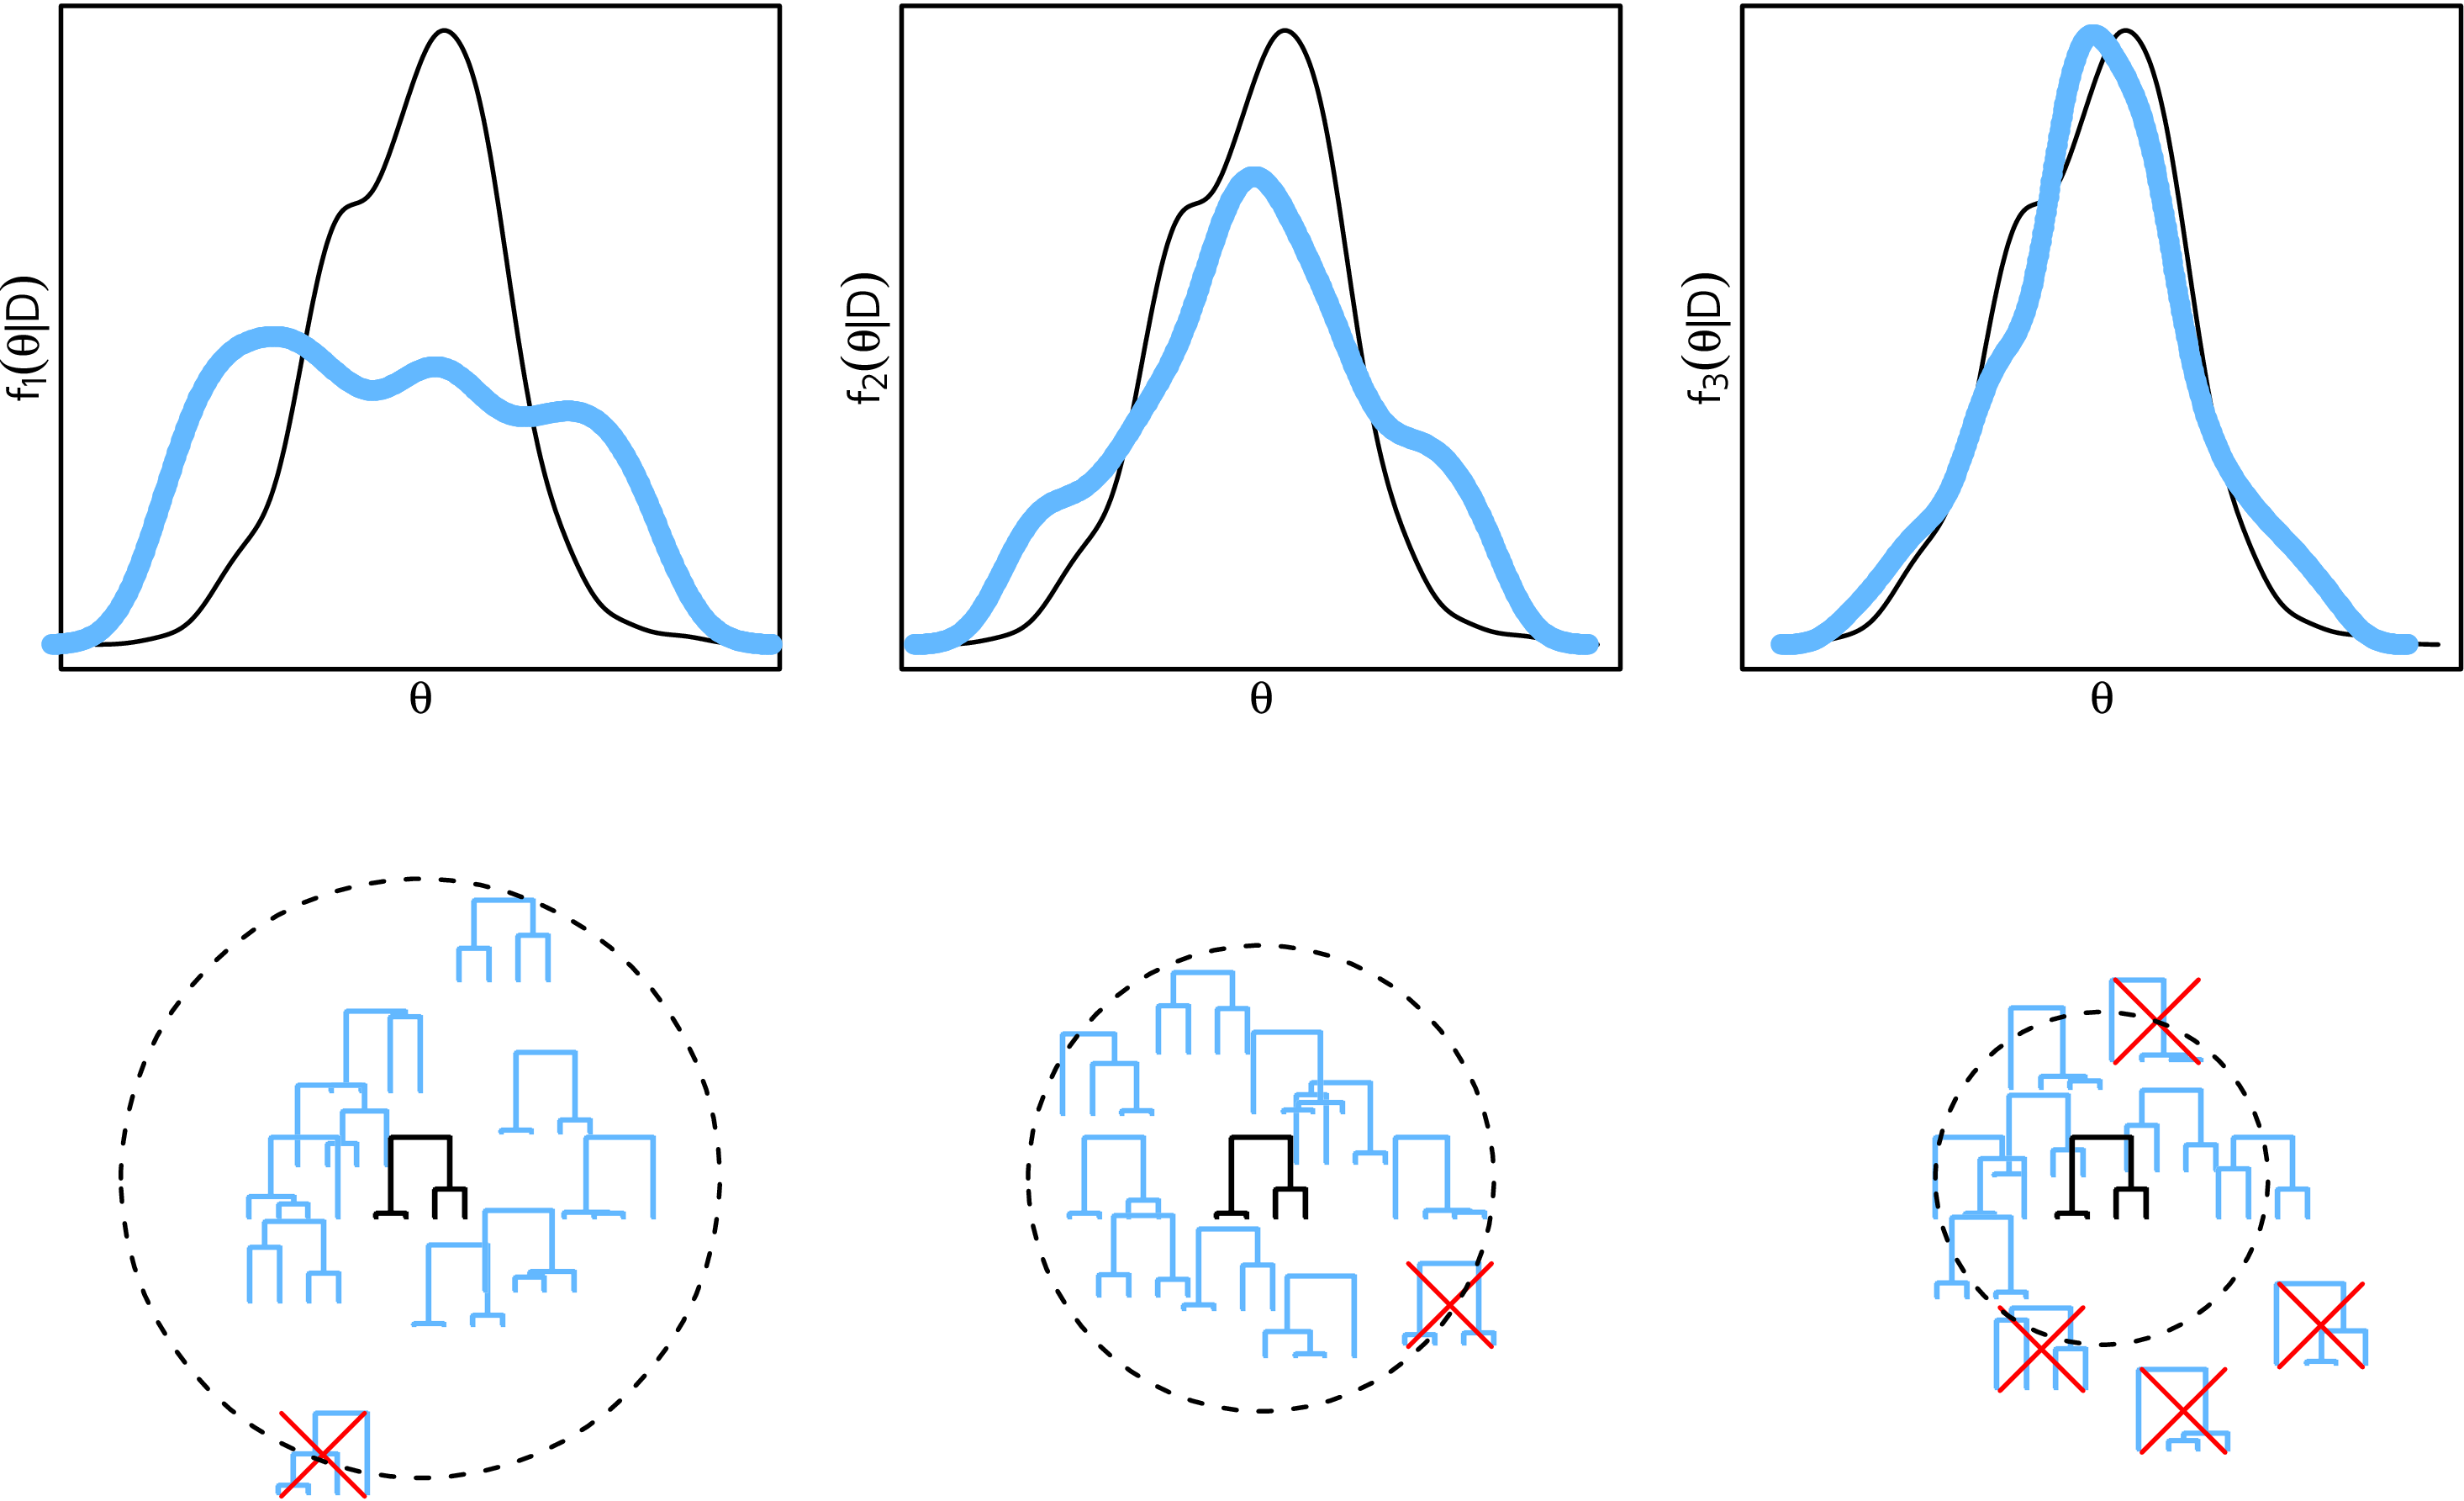
\includegraphics{abc-smc.pdf}
    \caption[Graphical schematic of the ABC-SMC algorithm implemented in \software{netabc}.]{
      Graphical schematic of the \gls{ABC}-\gls{SMC} algorithm implemented in
      \software{netabc}. Particles are initially drawn from their prior
      distributions, making the initial population a Monte Carlo approximation
      to the prior. At each iteration, particles are perturbed, and a distance
      threshold around the true tree contracts. Particles are rejected, and
      eventually resampled, when all their associated simulated trees lie
      outside the threshold. As the algorithm progresses, the population
      smoothly approaches a Monte Carlo approximation of the \gls{ABC} target
      distribution, which is assumed to resemble the posterior.
    }
    \label{fig:abcsmc}
\end{figure}

\software{Netabc} is written in the \software{C} programming language. The
\software{igraph} library~\autocite{csardi2006igraph} is used to generate and
store contact networks and phylogenies. Judy arrays~\autocite{baskins2004judy}
are used for hash tables and dynamic programming matrices. The
\gls{GSL}~\autocite{gough2009gnu} is used to generate random draws from
probability distributions, and to perform the bisection step in the adaptive
\gls{ABC}-\gls{SMC} algorithm. Parallelization is implemented with \gls{POSIX}
threads~\autocite{barney2009posix}. In addition to the \software{netabc} binary
to perform kernel-assisted \gls{ABC}, we provide three additional stand-alone
utilities: \software{treekernel}, to calculate the tree kernel;
\software{nettree}, to simulate a transmission tree over a contact network; and
\software{treestat}, to compute various summary statistics of phylogenies. The
programs are freely available at \url{https://github.com/rmcclosk/netabc}.

To check that our implementation of Gillespie simulation was correct, we
reproduced Figure 1A of \textcite{leventhal2012inferring} (our
\cref{fig:leventhal}), which plots the imbalance of transmission trees
simulated over four network models at various levels of pathogen
transmissibility. Our implementation of adaptive \gls{ABC}-\gls{SMC} was tested
by applying it to the same mixture of Gaussians used by
\textcite{del2012adaptive} to demonstrate their method (originally used
by~\textcite{sisson2007sequential}). We were able to obtain a close
approximation to the function (see \cref{fig:smctest}), and attained the
stopping condition used by the authors in a comparable number of steps. To
check that the algorithm would converge to a bimodal distribution, we also
applied it to a mixture of two Gaussians with means $\pm$4 and variances 1. The
algorithm was able to recover both peaks (\cref{fig:smctest2}).

\subsection{Simulation of transmission trees over contact networks}
\label{subsec:nettree}

The simulation of epidemics, and the corresponding transmission trees, over
contact networks is performed in \software{netabc} using the Gillespie
simulation algorithm~\autocite{gillespie1976general}. This method has been
independently implemented and applied by several
authors~\autocite[\textit{e.g.}][]{o2011contact, robinson2013dynamics,
leventhal2012inferring, groendyke2011bayesian, villandre2016assessment}.
\textcite{groendyke2011bayesian} published their implementation as an
\software{R} package, but since the \gls{SMC} algorithm is quite
computationally intensive, we chose to implement our own version in
\software{C} {\color{blue}\uline{as part of \software{netabc}}}.

Let $G = (V, E)$ be a directed contact network. We assume the individual nodes
and edges of $G$ follow the dynamics of the \gls{SIR}
model~\autocite{kermack1927contribution}. Each directed edge $e = (u, v)$ in
the network is associated with a transmission rate $\beta_e$, which indicates
that, once $u$ becomes infected, the waiting time until $u$ infects $v$ is
distributed as $\Exponential(\beta_e)$. Note that $v$ may become infected
before this time has elapsed, if $v$ has other incoming edges. $v$ also has a
removal rate $\gamma_v$, so that the waiting time until removal of $v$ from the
population is $\Exponential(\gamma_v)$. Removal may correspond to death or
recovery with immunity, or a combination of both, but in our implementation
recovered nodes never re-enter the susceptible population. We define a
\defn{discordant edge} as an edge $(u, v)$ where $u$ is infected and $v$ has
never been infected.

To describe the algorithm, we introduce some notation and variables. Let
$\inc(v)$ be the set of incoming edges to $v$, and $\out(v)$ be the set of
outgoing edges from $v$. Let $I$ be the set of infected nodes in the network,
$R$ be the set of removed nodes, and $S$ be the remaining susceptible nodes,
and $D$ be the set of discordant edges in the network. Let $\beta$ be the total
transmission rate over all discordant edges, and $\gamma$ be the total removal
rate of all infected nodes,
\[
  \beta = \sum_{e \in D} \beta_e, \quad
  \gamma = \sum_{v \in I} \gamma_v.
\]
The variables $S$, $I$, $R$, $D$, $\beta$, and $\gamma$ are all updated as the
simulation progresses. When a node $v$ becomes infected, it is deleted from $S$
and added to $I$. Any formerly discordant edges in $\inc(v)$ are deleted from
$D$, and edges in $\out(v)$ to nodes in $S$ are added to $D$. If $v$ is later
removed, it is deleted from $I$ and added to $R$, and any discordant edges in
$\out(v)$ are deleted from $D$. At the time of either infection or removal, the
variables $\beta$ and $\gamma$ are updated to reflect the changes in the
network. Since these updates are straightforward, we do not write them
explicitly in the algorithm.

\newcommand{\tip}{\mathit{tip}}

The Gillespie simulation algorithm is given as Algorithm~\ref{alg:nettree}. The
transmission tree $T$ is simulated along with the epidemic. We keep a map
called $\tip$, which maps infected nodes in $I$ to the tips of $T$. The
simulation continues until either there are no discordant edges left in the
network, or we reach a user-defined cutoff of time ($t_{\max}$) or number of
infections ($I_{\max}$). We use the notation $\Uniform(0, 1)$ to indicate a
number drawn from a uniform distribution on $(0, 1)$, and likewise for
$\Exponential(\lambda)$. The combined number of internal nodes and tips in $T$
is denoted $|T|$.

\begin{algorithm}
  \label{alg:nettree}
  \caption{Simulation of an epidemic and transmission tree over a contact network}
  \begin{algorithmic}
    \State infect a node $v$ at random, updating $S$, $I$, $D$, $\beta$ and $\gamma$
    \State $T \gets$ a single node with label $1$
    \State $\tip[v] \gets 1$
    \State $t \gets 0$
    \While{$D \neq \emptyset$ and $|I| + |R| < I_{\max}$ and $t < t_{\max}$}
      \State $s \gets \min(t_{\max} - t, \Exponential(\beta + \gamma))$
      \For{$v \in \tip$}
        \State{extend the branch length of $\tip[v]$ by $s$}
      \EndFor
      \State $t \gets t + s$
      \If{$t < t_{\max}$}
        \If{$\Uniform(0, \beta + \gamma) < \beta$}
          \State choose an edge $e = (u, v)$ from $D$ with probability $\beta_e / \beta$
                 and infect $v$
          \State $\tip[v] \gets |T|+1$
          \Comment{add new tips to tree and tip array}
          \State $\tip[u] \gets |T|+2$
          \Comment{corresponding to $u$ and $v$}
          \State add tips with labels $(|T|+1)$ and $(|T|+2)$ to $T$
          \State connect the new nodes to $\tip[v]$ in $T$, with branch lengths $0$
        \Else
          \State choose a node $v$ from $I$ with probability $\gamma_v / \gamma$
                 and remove $v$
          \State delete $v$ from $\tip$
        \EndIf
        \State update $S$, $I$, $R$, $D$, $\beta$, and $\gamma$
      \EndIf
    \EndWhile
  \end{algorithmic}
\end{algorithm}

\subsection{Phylogenetic kernel}

The tree kernel developed by \textcite{poon2013mapping} provides a
comprehensive similarity score between two phylogenetic trees, via the
dot-product of the two trees' feature vectors in the space of all possible
subset trees with branch lengths (see \cref{subsec:treeshape}). {\color{blue}
\uline{Because the branch lengths are continuous, there are infinitely many
possible subset trees; hence, the feature space is infinite-dimensional.}}
The kernel was implemented using the fast algorithm developed by
\textcite{moschitti2006making}. First, the production rule of each node, which
is the total number of children and the number of leaf children, is recorded.
The nodes of both trees are ordered by production rule, and a list of pairs of
nodes sharing the same production rule is created. These are the nodes for
which the value of the tree kernel must be computed - all other pairs have a
value of zero. The pairs to be compared are then re-ordered so that the child
nodes are always evaluated before their parents. Due to its recursive
definition, ordering the pairs in this way allows the tree kernel to be
computed by dynamic programming. The complexity of this implementation is
$O(|T_1||T_2|)$ for the two trees $T_1$ and $T_2$ being compared.

The tree kernel cannot be used directly as a distance measure for \gls{ABC},
since it is maximized, not minimized, when the two trees being compared are the
same. Therefore, we defined the distance between two trees as
\[
  \rho(T_1, T_2) = 1 - \frac{K(T_1, T_2)}{\sqrt{K(T_1, T_1) K(T_2, T_2)}},
\]
which is a number between 0 and 1 that is minimized when $T_1 = T_2$. This is
similar to the normalization used by \textcite{collins2002new,
poon2013mapping}.

\subsection{Adaptive sequential Monte Carlo for Approximate Bayesian computation}
\label{subsec:adaptsmc}

We implemented the adaptive \gls{SMC} algorithm for \gls{ABC} developed by
\textcite{del2012adaptive}. This algorithm is similar to the reference
\gls{ABC}-\gls{SMC} algorithm described in \cref{subsec:abcalg}, except that
the sequence of tolerances $\varepsilon_i$ is automatically determined rather
than specified in advance. The tolerances are chosen such that the \gls{ESS} of
the particle population, which indicates the quality of the Monte Carlo
approximation (see \cref{subsec:sis}), decays at a controlled rate. A
sudden precipitous drop in \gls{ESS} would indicate that only a small number of
particles had non-zero importance weights, which would result in a very poor
Monte Carlo approximation to the target distribution. This situation is
referred to as the ``collapse'' of the approximation, {\color{blue}\uline{also
known as particle degeneracy} (see \cref{subsec:smc})} and is mitigated by the
adaptive approach. A single parameter {\color{red}\sout{$\alpha$ (not to be
confused with the \gls{BA} model parameter)}} controls the decay rate.
{\color{blue}\uline{In the original paper of }\textcite{del2012adaptive},
\uline{the parameter is called $\alpha$, but to avoid confusion with the
\gls{BA} parameter of the same name, we will refer to it here as
\gls{alphaess}.}}
The tolerance $\varepsilon_i$ is chosen to satisfy
\[
  \ESS(w_i) = \alpha_{\ESS} \ESS(w_{i-1}),
\]
where, $w_i$ is the vector of weights at the $i$th step. Note that, since $w_i$
depends on $\varepsilon_i$, this equation solves for the updated weights and
the updated tolerance simultaneously. As pointed out by
\textcite{del2012adaptive}, the equation has no analytic solution, but can be
solved numerically by bisection. The forward kernels $K_i$ are taken to be
\gls{MCMC} kernels with stationary distributions $\pi_{\varepsilon_i}$ and
proposal distributions
\[
  q_i(\theta, \theta') \prod_{k=1}^M \Pr(z_i^{(k)'} \mid \theta'),
\]
where $\theta$ is the vector of model parameters and $z_k$ are $M$ datasets
simulated according to $\theta'$. In our implementation, $q$ is either a
Gaussian proposal for continuous parameters, or a Poisson proposal for discrete
parameters. For the Poisson proposals, the number of steps to move the particle
is drawn from a Poisson distribution, and the direction in which to move the
particle is chosen uniformly at random. For both proposals, the variance was
set equal to twice the empirical variance of the particles,
following~\autocite{beaumont2009adaptive, del2012adaptive}. The backwards
kernels are
\[
  L_{i-1}(x', x) = \frac{\pi_n(x)K(x, x')}{\pi_n(x')}.
\]
When substituted into \cref{eq:smcwt}, the forward kernels $K(x, x')$ and
densities $\pi_n(x') = \pi_{\varepsilon_n}(x')$ cancel out, and we are left
with the weight update 
\begin{align*}
  w_i(x) 
    &\propto w_{i-1}(x) \frac{\pi_n(x \mid y)}{\pi_{i-1}(x \mid y)} \\
    &= w_{i-1}(x) \frac{\pi(x) \pi_i(y \mid x)}{\pi(x) \pi_{i-1}(y \mid x)} \\
    &= w_{i-1}(x) \frac{\sum_{k=i}^M \I_{A_{\varepsilon_i, y}}(z_k)}
            {\sum_{k=i}^M \I_{A_{\varepsilon_{i-1}, y}}(z_k)}.
\end{align*}
In other words, when the distance threshold $\varepsilon_{i-1}$ is contracted
to $\varepsilon_i$, the particles' weights are multiplied by the proportion of
simulated datasets that are still inside the new threshold. 
The user may specify a final tolerance $\varepsilon$, or a final acceptance
rate of the \gls{MCMC} kernel, and the algorithm will be stopped when either of
these termination conditions is reached. The latter condition stops the
algorithm when the particles are not moving around very much, implying little
change in the estimated target.

\subsection{Justification for approach}
\label{subsec:just}

{\color{blue}\uline{We present here a non-rigorous justification for the use of
\gls{ABC} for the problem at hand, as opposed to more frequently-used
approaches for fitting mathematical models} (see \cref{chp:prelim}).
\uline{Consider a contact network model with parameters $\theta$, and an
estimated transmission tree $T$. Taking a Bayesian approach, our aim is to
obtain a sample from the posterior distribution on the model's parameters given
our data,}
\[
    \Pr(\theta \mid T) = \frac{\Pr(T \mid \theta) \Pr(\theta)}{\Pr(T)}.
\]
\uline{For all but the simplest models, the normalizing constant $\Pr(T)$ is an
intractable integral. What we shall argue here is that, in contrast to most
commonly studied mathematical models, the likelihood $\Pr(T \mid \theta)$ is
also likely to be intractible in our case.}

\begin{figure}
    \centering
    \includegraphics[width=\textwidth]{transtree}
    \caption[
        Illustration of an estimated transmission tree without labels and two
        possible underlying complete transmission trees with labels.
    ]{
        Illustration of an estimated transmission tree without labels (left)
        and two possible underlying complete transmission trees with labels
        (right). In the top right scenario, the epidemic began with node $a$
        who transmitted first to $b$ and then to $c$. In the bottom right
        scenario, $b$ was the index case; $b$ infected $c$, who went on to
        infect $a$. A transmission tree estimated from a viral phylogeny would
        have the same topology and tip labels in both cases.
    }
    \label{fig:tt}
\end{figure}

\uline{As discussed in} \cref{subsec:tt}, \uline{the internal nodes of
transmission trees represent transmission events, and are labelled with the
donor in the associated transmission pair. However, when we estimate a
transmission tree from viral sequence data, we generally only know the labels
of the tips of the tree, not the labels of the internal nodes. In viral
phylogenies, the transmissions are at least partially preserved through the
evolutionary relationships among the viruses, but the directionality of those
transmissions is unknown. Thus, a single estimated transmission tree can
correspond to many possible pathways of the epidemic through the network.
}\Cref{fig:tt} \uline{illustrates this concept for a simple transmission tree
with three tips. When calculating a likelihood given a transmission tree, we
must sum over all possible labellings of the internal nodes. Let $\Nu$ be the
set of such labellings. Then}
\begin{align}
    \Pr(T \mid \theta) = \sum{\nu \in \Nu} \Pr(T, \nu \mid \theta).
    \label{eq:lik1}
\end{align}
\uline{A contact network model assigns a probability to each possible contact
network. Transmission trees are realized over particular contact networks, not
over the model itself. Therefore, we must also sum over all contact networks
which could be generated by the model. Let $\G$ be the set of all possible
contact networks. Summing } \cref{eq:lik1} \uline{over $\G$ gives}
\begin{align}
    \Pr(T \mid \theta) = \sum_{G \in \G} \sum{\nu \in \Nu} 
        \Pr(T, \nu \mid G, \theta) \Pr(G \mid \theta).
    \label{eq:lik2}
\end{align}
\uline{This can be simplified somewhat by noticing that, given a specific
contact network, the labelled transmission tree depends only on that network
and not on the model that generated it. That is, $\Pr(T, \nu \mid G, \theta) =
\Pr(T, \nu \mid G)$, and}
\begin{align}
    \Pr(T \mid \theta) = \sum_{G \in \G} \Pr(G \mid \theta) \sum{\nu \in \Nu} 
        \Pr(T, \nu \mid G)
    \label{eq:lik3}
\end{align}
\uline{Under the assumption that both transmission and removal are Poisson
processes, calculating $\Pr(T, \nu \mid G)$ can be accomplished by a
straightforward modification of the Gillespie simulation algorithm} 
(\cref{alg:nettree}). \uline{Rather than choosing transmission or removal
events according to their probabilities, the events would be deterministically
chosen based on the transmission tree and the probabilities of each event
would be multiplied together. Assuming efficient data structures for storing
lists of nodes and edges, the complexity of this calculation would be $O(|T|)$.
The number of possible labellings of internal nodes of $T$ is easily seen to be
$2^{(|T|-1)/2}$ by noticing that each of the $(|T|-1)/2$ internal nodes must be
labelled with the same label as either its right child or its left child.
Although exponential calculations of this nature can are often be simplified on 
trees using dynamic programming} (\eg \autocite{pupko2000fast}), \uline{it
cannot be straightforwardly applied in this case because the subtrees'
probabilities depend on the existing epidemic progress (their parents and
siblings). Hence, calculating the inner sum over labels may take time
$O(2^{(|T|-1)/2})$.}

\uline{The outer sum, over all contact networks, is also difficult to evaluate
in general. There are $2^{N(N-1)}$ directed graphs on $N$
nodes~\autocite{harary2014graphical}. There must be at least as many nodes in
the contact network as the number of tips in the tree, which is $(|T|+1)/2$. Of
course, it is very likely that there are more nodes in the network than
observed tips because some individuals are never infected and/or some infected
individuals are never sampled. The complexity of calculating $\Pr(G \mid
\theta)$ is obviously dependent on the particular model being investigated. For
the \gls{BA} model, we might have to sum over all possible orders in which the
nodes could be added, and all assignments of edges to the nodes which generated
them. However, even in the unlikely case that calculating $\Pr(G \mid \theta)$
can be done in constant time, the sum} \ref{eq:lik3} \uline{still has at least
$O(2^{|T|^2})$ terms.}

\uline{We have shown that both the normalizing constant $\Pr(T)$ and the
likelihood $\Pr(T \mid \theta)$ are likely computationally prohibitive to
calculate. If this is the case, the problem of fitting contact network models
to phylogenies seems to be of the \emph{doubly-intractible}
ype~\autocite{murray2012mcmc}, which would imply that these models are not
amenable to neither \gls{ML} nor Bayesian inference techniques. Although both
methods are able to cope with an intractible normalizing constant (for example,
by local search for \gls{ML} or Bayesian \gls{MCMC}), neither can avoid the
intractable likelihood calculations. This justifies the use of \gls{ABC}, which
is a likelihood-free method.}

\uline{We have not proven here that} \cref{eq:lik3} \uline{is impossible to
calculate in polynomial time - it could be possible to algebraically simplify
the sum into a tractable expression. Furthermore, under certain models, a large
proportion of $\G$ may have zero probability, which would enable the
simplification of the outer sum on a model-specific basis. It should also be
noted that extensions of Bayesian \gls{MCMC} have been developed for
doubly-intractable problems~\autocite{liang2010double, murray2012mcmc}, which
might be adaptable to the problem at hand. These have not been as widely used
as \gls{ABC}, nor are they as easily parallelizable as \gls{SMC}. }}

\section{Analysis of \acrlong{BA} model with synthetic data}
\label{sec:ba}

\subsection{Methods}
\glsreset{BA}

%{\color{blue}\uline{The \gls{BA} contact network model} (see \cref{subsec:pa})
%\uline{generates networks with a power law degree distribution. Power law
%distributions have been observed by several empirical studies of sexual
%behaviour}~\autocite{colgate1989risk, liljeros2001web, schneeberger2004scale,
%clemencon2015statistical} (although not all, see
%\autocite{handcock2004likelihood, bansal2007individual}).}

{\color{blue}\uline{Using synthetic data,}} we investigated four parameters
related to the \gls{BA} contact network model, denoted \gls{N}, \gls{m},
\gls{alpha}, \gls{I} (see \cref{subsec:pa}). The first three of these are
parameters of the model itself, while \gls{I} is related to the simulation of
transmission trees over the network. However, we will refer to all four as
\gls{BA} parameters. \gls{N} denotes the total number of nodes in the network,
or equivalently, susceptible individuals in the population. When a node is
added to the network, \gls{m} new undirected edges are added incident to it,
and are attached to existing nodes of degree $k$ with probability proportional
to $k^\alpha + 1$ (\cref{subsec:pa}). To simulate transmission trees over a
\gls{BA} network, we allowed an epidemic to spread until \gls{I} nodes were
infected, and sampled a transmission tree at that time. The \gls{alpha}
parameter is unitless, while \gls{m} has units of edges or connections per
vertex, and \gls{N} and \gls{I} both have units of nodes or individuals.

{\color{blue}\uline{Our investigation comprised three sets of computational
experiments aimed at determining which of these parameters could be estimated
from phylogenetic data, and with what degree of accuracy. First, we performed
an exploratory analysis using a tree kernel-based classifier to determine which
of the four \gls{BA} parameters might be identifiable from tree shapes when all
others were held fixed. This analysis was also used to validate our choice of
the tree kernel as a distance function for \gls{ABC}, by evaluating two further
classifiers based on other tree summary statistics from the literature. Second,
we used grid search to investigate the accuracy and precision of marginal
parameter estimates, again holding all but one parameters of the model fixed.
Finally, we applied the full \gls{ABC}-\gls{SMC} algorithm to jointly estimate
the four parameters of the \gls{BA} model simultaneously.}}

We assumed that all contacts had symmetric transmission risk, which was
implemented by replacing each undirected edge in the network with two directed
edges (one in each direction). Nodes in our networks followed simple \gls{SI}
dynamics, meaning that they became infected at a rate proportional to their
number of infected neighbours, and never recovered. We did not consider the
time scale of the transmission trees in these simulations, only their shape.
Therefore, the transmission rate along each edge in the network was set to 1,
the removal rate of each node was set to 0, and all transmission trees' branch
lengths were scaled by their mean. The \textit{igraph} library's implementation
of the BA model~\autocite{csardi2006igraph} was used to generate the graphs.
The analyses were run on Westgrid (\url{https://www.westgrid.ca/}) and a local
computer cluster. With the exception of our own programs, all analyses were
done in \software{R}, and all packages listed below are \software{R} packages.
{\color{blue}\uline{Code to run all simulation-based experiments is freely
available at \url{https://github.com/rmcclosk/thesis}.}}

\subsubsection*{Classifiers for BA model parameters based on tree shape}
\label{subsec:kernel}

\glsreset{nltt}

{\color{blue}\uline{
Our first computational experiment was designed as an exploratory analysis of
the four \gls{BA} model parameters defined above: \gls{alpha}, \gls{I},
\gls{m}, and \gls{N}. The objective of this experiment was to determine whether
any of the four parameters were identifiable from the shape of the transmission
tree, as quantified by the tree kernel. Each of the \gls{BA} model parameters
was varied one at a time, while holding the other parameters at fixed, known
values. Contact networks were generated according to each set of parameter
values, and transmission trees were simulated over the networks. We then
evaluated how well a classifier based on the tree kernel could differentiate
the trees simulated under distinct parameter values. If the classifier's
cross-validation accuracy was high, this could be taken as an indication that
the parameter in question was identifiable in the range of values considered. 
A caveat of this preliminary analysis is that, since all parameters but one
were held at known values, nothing could be said about the identifiability of
\emph{combinations} of parameters; this issue will be explored later by jointly
estimating all parameters with \gls{ABC}}.

\uline{In addition to testing for identifiability, a secondary objective of
this analysis was to validate the use of the tree kernel as a distance measure
for \gls{ABC} in our context. As discussed in} \cref{sec:abc}, \uline{the
choice of distance function is extremely important for the accuracy of the
\gls{ABC} approximation to the posterior. Therefore, we evaluated two
additional tree statistics in the same manner as we evaluated the tree kernel
(that is, by constructing and testing a classifier). First, we considered
Sackin's index~\autocite{shao1990tree}, which measures the degree of imbalance
or asymmetry in a phylogeny} (see \cref{subsec:treeshape}). \uline{Sackin's
index is widely used for characterizing
phylogenies~\autocite{frost2013modelling} and has been demonstrated to vary
between transmission trees simulated under different contact network
types~\autocite{leventhal2012inferring}. Sackin's index does not take branch
lengths into account, considering only the tree's topology. The other statistic
we considered was the \gls{nltt}~\autocite{janzen2015approximate}, which
compares two trees based on normalized distributions of their branching times}
(see \cref{subsec:treeshape}).  \uline{In contrast with Sackin's index, the
\gls{nltt} does not explicity consider the trees' topologies, but it does use
their normalized branch lengths. While the \gls{nltt} is a newly developed
statistic not yet in widespread use, the unnormalized
\gls{ltt}~\autocite{nee1992tempo} was the basis of seminal early work
extracting epidemiological information from
phylodynamics~\autocite{holmes1995revealing}. We expected the tree kernel to
classify the \gls{BA} parameters more accurately than either Sackin's index or
the \gls{nltt}, since the tree kernel takes both topology and branch lengths
into account. }}

This experiment involved a large number of variables that were varied
combinatorially. For ease of exposition, we will describe a single experiment
first, then enumerate the values of all variables for which the experiment was
repeated. The parameters of the tree kernel, $\lambda$ and $\sigma$
(\cref{subsec:treeshape}), will be referred to as \defn{meta-parameters} to
distinguish them from the parameters of the \gls{BA} model. 

The attachment power parameter \gls{alpha} was varied among three values: 0.5,
1.0, and 1.5. For each value, the \software{sample\_pa} function in the
\software{igraph} package was used to simulate 100 networks, with the other
parameters set to \gls{N} = 5000 and \gls{m} = 2. This step yielded a total of
300 networks. An epidemic was simulated on each network using our
\software{nettree} binary until \gls{I} = 1000 nodes were infected, at which
point 500 of them were sampled to form a transmission tree. A total of 300
transmission trees were thus obtained, comprised of 100 trees for each of the
three values of \gls{alpha}. The trees were ``ladderized'' so that the subtree
descending from the left child of each node was not smaller than that
descending from the right child. Summary statistics, such as Sackin's index and
the ratio of internal to terminal branch lengths, were computed for each
simulated tree using our \software{treestat} binary. The trees were visualized
using the \software{ape} package~\autocite{paradis2004ape}. {\color{blue}\uline{
Both the tree kernel and the \gls{nltt} are pairwise statistics, and the
\glspl{SVM} classifiers we used to investigate them operate on pairwise
distance matrices.}} Our \software{treekernel} binary was used to calculate the
value of the kernel for each pair of trees, with the meta-parameters set to
$\lambda = 0.3$ and $\sigma = 4$. These values were stored in a symmetric 300
$\times$ 300 kernel matrix.  Similarly, we computed the \gls{nltt} statistic
between each pair of trees using our \software{treestat} binary, and stored
them in a second $300 \times 300$ matrix.

To investigate the identifiability of \gls{alpha} from tree shape, we
constructed classifiers for \gls{alpha} based on the three tree shape
statistics discussed above. First, we used the \software{kernlab}
package~\autocite{zeileis2004kernlab} to create a \gls{kSVR} classifier using
the computed kernel matrix. Second, we used the \software{e1071}
package~\autocite{meyer2015e1071} to create an ordinary \gls{SVR} classifier
using the pairwise \gls{nltt} matrix. Finally, we performed an ordinary linear
regression of \gls{alpha} against Sackin's index. Each of these classifiers was
evaluated with 1000 two-fold cross-validations. We also performed a \gls{kPCA}
projection of the kernel matrix, and used it to visualize the separation of the
different \gls{alpha} values in the tree kernel's feature space. A schematic of
this experiment is presented in \cref{fig:kernelexpt}.

Similar experiments were performed with the values shown in
\cref{tab:kernelexpt}. The other three \gls{BA} parameters, namely \gls{N},
\gls{m}, and \gls{I}, were each varied while holding the others fixed. The
experiments for \gls{alpha}, \gls{m}, and \gls{N} were repeated with three
different values of \gls{I}. All experiments were repeated with trees having
three different numbers of tips. Kernel matrices were computed for all pairs of
the meta-parameters \gls{lambda} = \sett{0.2, 0.3, 0.4} and \gls{sigma} =
\sett{\nicefrac18, \nicefrac14, \nicefrac12, 1, 2, 4, 8}.

\begin{landscape}
\begin{table}[ht]
  \centering
  \documentclass{article}

\usepackage{tikz}
\usepackage{array}
\usepackage{nicefrac}
\usepackage{fullpage}
\usepackage[T1]{fontenc}
\usepackage[sfmath]{kpfonts}
\usepackage[default]{gillius}
\usepackage[normalem]{ulem}

\usetikzlibrary{positioning}
\usetikzlibrary{arrows}
\usetikzlibrary{calc}

\begin{document}
\immediate\write18{./kernel-expt-extra.R}

\pagestyle{empty}

\newcommand{\boxw}{7cm}
\newcommand{\boxh}{2cm}

\begin{tikzpicture}
  \tikzstyle{box}=[minimum width=\boxw, minimum height=\boxh, draw]
  \tikzstyle{next}=[->, >=stealth, thick]

  \node (rect1) [box] { };
  \node at (rect1.north) [anchor=north] {\uline{3 parameter values}};
  \node (b) [above=0.5cm of rect1.south, blue] {\LARGE $\theta_1$};
  \node (r) [left=1.5cm of b, red] {\LARGE $\theta_2$};
  \node (g) [right=1.5cm of b, green] {\LARGE $\theta_3$};

  \node (rect2) [below=of rect1, box] { };
  \node at (rect2.north) [anchor=north] {\uline{300 networks}};
  \node (b) [above=4pt of rect2.south] {
    \begin{tabular}{m{0.5cm} m{1cm} m{0.5cm} m{1cm} m{0.5cm} m{1cm}}
      
\includegraphics[width=1cm]{tinynet1} & $\times$ 100 &
      
\includegraphics[width=1cm]{tinynet2} & $\times$ 100 &
      
\includegraphics[width=1cm]{tinynet3} & $\times$ 100
    \end{tabular}
  };

  \node (rect3) [below=of rect2, box] { };
  \node at (rect3.north) [anchor=north] {\uline{300 epidemics}};
  \node (b) [above=4pt of rect3.south] {
    \begin{tabular}{m{0.5cm} m{1cm} m{0.5cm} m{1cm} m{0.5cm} m{1cm}}
      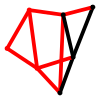
\includegraphics[width=1cm]{tinyepi1} & $\times$ 100 &
      
\includegraphics[width=1cm]{tinyepi2} & $\times$ 100 &
      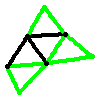
\includegraphics[width=1cm]{tinyepi3} & $\times$ 100
    \end{tabular}
  };

  \node (rect4) [below=of rect3, box] { };
  \node at (rect4.north) [anchor=north] {\uline{300 transmission trees}};
  \node (b) [above=4pt of rect4.south] {
    \begin{tabular}{m{0.5cm} m{1cm} m{0.5cm} m{1cm} m{0.5cm} m{1cm}}
      
\includegraphics[width=1cm]{tinytree1} & $\times$ 100 &
      
\includegraphics[width=1cm]{tinytree2} & $\times$ 100 &
      
\includegraphics[width=1cm]{tinytree3} & $\times$ 100
    \end{tabular}
  };

  \node (rect5) [right=of rect1, box] { };
  \node at (rect5.north) [anchor=north, text width=\boxw, align=center] {
    \uline{42 kernel matrices ($300 \times 300$)} \\ \vspace{4pt}
    $\lambda$ = \{ \nicefrac18, \nicefrac14, \nicefrac12, 1, 2, 4, 8 \} \\
    $\sigma$ = \{ 0.2, 0.3, 0.4 \} \\
    nLTT = \{ yes, no \} \\
  };

  \node (rect6) [below=of rect5, box] { };
  \node at (rect6.north) [anchor=north, text width=\boxw, align=center] {
    \uline{42 cross validations} \\ \hfill \\
    R$^2$ $\times$ 42
  };

  \node (rect7) [below=of rect6, box] { };
  \node at (rect7.north) [anchor=north, text width=\boxw, align=center] {
    \uline{optimal kernel meta-parameters} \\ \hfill \\
    $\lambda$ = 4,\; $\sigma$ = 0.3,\; nLTT = no
  };

  \node (rect8) [below=of rect7, minimum width=\boxw, minimum height=\boxh,
                 align=center, text width=\boxw] {
    repeat 8 times \\
    \vspace{4pt}
    infected nodes = \{ 500, 1000, 2000 \} \\
    sampled nodes = \{ 100, 500, 1000 \}
  };

  \coordinate [left=0.5 of rect5.west] (r5w);
  \coordinate [below=0.5cm of r] (r1ssw);
  \coordinate [below=of r1ssw] (r2nnw);
  \coordinate [below=0.5cm of g] (r1sse);
  \coordinate [below=of r1sse] (r2nne);
  \coordinate [below=3.5cm of r] (r2ssw);
  \coordinate [below=3.5cm of g] (r2sse);
  \coordinate [below=4.5cm of r] (r3nnw);
  \coordinate [below=4.5cm of g] (r3nne);
  \coordinate [below=6.5cm of r] (r3ssw);
  \coordinate [below=6.5cm of g] (r3sse);
  \coordinate [below=7.5cm of r] (r4nnw);
  \coordinate [below=7.5cm of g] (r4nne);
  \coordinate [below=0.5cm of rect4.north east] (r4ene);
  \coordinate [above=0.5cm of rect4.south east] (r4ese);

  \draw[next] (r1ssw) -- (r2nnw);
  \draw[next] (r1ssw) -- ($(r2nnw) + (-0.5cm, 0cm)$);
  \draw[next] (r1ssw) -- ($(r2nnw) + (0.5cm, 0cm)$);
  \draw[next] (r1sse) -- (r2nne);
  \draw[next] (r1sse) -- ($(r2nne) + (-0.5cm, 0cm)$);
  \draw[next] (r1sse) -- ($(r2nne) + (0.5cm, 0cm)$);
  \draw[next] (rect1.south) -- (rect2.north);
  \draw[next] (rect1.south) -- ($(rect2.north) + (-0.5cm, 0cm)$);
  \draw[next] (rect1.south) -- ($(rect2.north) + (0.5cm, 0cm)$);
  \draw [next] (rect2) -- (rect3);
  \draw [next] (r2ssw) -- (r3nnw);
  \draw [next] (r2sse) -- (r3nne);
  \draw [next] (rect3) -- (rect4);
  \draw [next] (r3ssw) -- (r4nnw);
  \draw [next] (r3sse) -- (r4nne);
  \draw [next] (rect4.east) -| (r5w) -- (rect5);
  \draw [thick] (r4ene) -- ++ (0.5cm, -0.5cm);
  \draw [thick] (r4ese) -- ++ (0.5cm, 0.5cm);
  \draw [next] (rect5) -- (rect6);
  \draw [next] (rect6) -- (rect7);
\end{tikzpicture}

\end{document}

  \caption[Variables used in tree kernel simulation experiments]
  {
    Values of parameters and other variables used in tree kernel simulation
    experiments. Each row corresponds to one of the \gls{BA} model parameters.
    One kernel matrix was created for every combination of values except the
    one indicated in the ``varied parameter'' column, which was varied when
    producing simulated trees.
  }
  \label{tab:kernelexpt}
\end{table}

\begin{table}[ht]
  \centering
  \begin{tabular}{cccccccc}
  parameter & grid values & test values & $N$ & $\alpha$ & $m$ & $I$ & tips \\
  \hline
  $N$ & 1050, 1125, \ldots, 15000 & 1000, 3000, \ldots, 15000 & - & 1.0 & 2 & 1000 & 100, 500, 1000 \\
  $\alpha$ & 0, 0.01, \ldots, 2 & 0, 0.25, \ldots 2 & 5000 & - & 2 & 1000 & 100, 500, 1000 \\
  $m$ & 1, 2, \ldots, 6 & 1, 2, \ldots 6 & 5000 & 1.0 & - & 1000 & 100, 500, 1000 \\
  $I$ & 500, 525, \ldots, 5000 & 500, 1000, 1500, 2000 & 5000 & 1.0 & 2 & - & 100, 500 \\
  \hline
\end{tabular}

  \caption[Variables used in grid search experiments]
  {
    Variables and \gls{BA} parameter values used for grid search experiments. 
    Trees were simulated under the test values, and compared to a grid of trees
    simulated under the grid values. Kernel scores were used to calculate point
    estimates and credible intervals for the test values.
  }
  \label{tab:gridexpt}
\end{table}
\end{landscape}

\begin{figure}[ht]
  \centering
  \includegraphics{kernel-expt.pdf}
  \caption[Schematic of experiments investigating impact of BA model parameters
           on tree shape.]{
    Schematic of experiments designed to investigate the impact of variations
    in BA model parameters on transmission tree shapes. The parameters of the
    BA model were varied one at a time {\color{blue}\uline{while holding all
    others fixed}}. Transmission trees were simulated under three different
    values of each parameter, then compared pairwise using the tree kernel.
    Classifiers were constructed for each parameter, and their accuracy was
    evaluated by cross-validation. Kernel-PCA projections were used to visually
    examine the separation of the trees in the feature space defined by the
    tree kernel.
  }
  \label{fig:kernelexpt}
\end{figure}

\subsubsection*{Grid search}

{\color{blue}\uline{The previous experiment was an exploratory analysis
intended to determine which of the \gls{BA} parameters were identifiable, and
whether the tree kernel could potentially be used to distinguish different
parameter values when all others were held fixed. In this experiment, which was
still of an exploratory nature, we continued to consider one parameter at a
time while fixing the other three. However, rather than checking for
identifiability, we were now interested in quantifying the accuracy and
precision of kernel score-based estimates. This was done by examining the
distribution of kernel scores on a grid of parameter values, when trees
simulated according to those values were compared with a single simulated test
tree. This experiment did not involve the full \gls{ABC}-\gls{SMC} algorithm,
nor did we continue to use Sackin's index or the \gls{nltt}.}}

As in the previous section, we will begin by describing a single experiment,
and then list the variables for which similar experiments were performed. We
varied \gls{alpha} along a narrowly spaced grid of values: 0, 0.01, \ldots, 2.
For each value, fifteen networks were generated with \software{igraph}, and
transmission trees were simulated over each using \software{nettree}. These
trees will be referred to as ``grid trees''. Next, one further test tree was
simulated with the test value \gls{alpha} = 0. Both the grid trees and the test
tree had 500 tips, and were simulated with the other \gls{BA} parameters set to
{\color{blue}\uline{the known values}} $N$ = 5000, $m$ = 2, and $I$ = 1000. The
test tree was compared to each of the grid trees using the tree kernel, with
the meta-parameters set to $\lambda = 0.3$ and $\sigma = 4$, using the
\software{treekernel} binary. The median kernel score was calculated for each
grid value, and the scores were normalized such that the area under the curve
was equal to 1. {\color{red}\sout{The grid value with the highest median kernel
score was taken as the point estimate for the test value}}{\color{blue}\uline{
A point estimate for the test value was obtained by calculating the weighted
mean of the grid values with the kernel scores as weights}}, and a 95\%
credible interval was obtained using the \software{hpd} function in the
\software{TeachingDemos} package~\autocite{snow2013teachingdemos}.

Each experiment of the type just described was repeated ten times with the same
test value. Similar experiments were performed for each of the four \gls{BA}
parameters, with several test values and trees of varying sizes. The variables
are listed in \cref{tab:gridexpt}. A graphical schematic of the grid search
experiments is shown in \cref{fig:gridexpt}. {\color{blue}\uline{We emphasize
that these experiments were marginal in nature; that is, the each parameter was
varied and estimated individually while holding the others at known, fixed
values.}}

%Spearman's correlation was used to test whether the number of tips in the tree
%was correlated with the acccuracy of the point estimates. One-way \gls{ANOVA}
%was used to test whether the accuracy of the point estimates were significantly
%higher for any parameter values. If so, the distribution of errors was examined
%to choose a suitable post hoc test. If there appeared to be a correlation
%between the parameter value and the accuracy of the estimate, Spearman's
%correlation was calculated. If there were one or more particular values which
%appeared to have lower error, we used the Wilcoxon rank-sum test.

\begin{figure}[ht]
  \centering
  \includegraphics[width=\textwidth]{gridsearch-expt}
  \caption[Schematic of grid search experiment.]{
    Graphical schematic of grid search experiments used to investigate \gls{BA}
    model parameters. Trees were simulated along a narrowly spaced grid of
    values of one parameter (``grid trees'') {\color{blue}\uline{with all other
    parameters fixed to known values}}. Separate trees were simulated for a
    small subset of the grid values (``test trees''), {\color{blue}\uline{also
    holding the other parameters fixed}}. Each test tree was
    compared to every grid tree using the tree kernel, and the resulting kernel
    scores were normalized to resemble a probability density from which the
    mode and 95\% highest density interval were calculated.
  }
  \label{fig:gridexpt}
\end{figure}

\subsubsection*{Approximate Bayesian computation}

{\color{blue}\uline{
Our final simulation-based experiment was designed to test the full
\gls{ABC}-\gls{SMC} algorithm by jointly estimating the four parameters of the
\gls{BA} model. In contrast to the previous two experiments, we did not inform
the algorithm of any of the true parameter values.  }}

We simulated three trees each under a variety of parameter values and ran the
\software{netabc} program to estimate posterior distributions for the
parameters. The parameter values and priors used are listed in
\cref{tab:abcexpt}. The tree kernel meta-parameters were set to $\lambda = 0.3$
and $\sigma = 4$. The \gls{SMC} algorithm was run with 1000 particles, five
sampled datasets per particle, and the $\alpha_{\ESS}$ parameter (not to be
confused with the \gls{BA} preferential attachment parameter, see
\cref{subsec:adaptsmc}) set to 0.95. The algorithm was stopped when the
acceptance rate of the \gls{MH} kernel dropped below 1.5\%, the same criterion
used by \citeauthor{del2012adaptive}. Approximate marginal posterior densities
for each parameter were calculated using the \software{density} function in
\software{R} applied to the final weighted population of particles.
{\color{red}\sout{Credible intervals were obtained for each parameter using the
\software{HPDinterval} function in the \software{coda}
package~\autocite{plummer2006coda}.}} {\color{blue}\uline{Posterior means
obtained for each parameter using the \software{wtd.mean} function in the
\software{Hmisc} package~\autocite{harrell2016hmisc}. Credible intervals were
obtained using the \software{hpd} function in the \software{TeachingDemos}
package~\autocite{snow2013teachingdemos}.}}

\begin{table}[ht]
  \centering
  \begin{tabular}{ccc}
  parameter or variable & test values & prior \\
  \hline
  $N$ & 5000 & Uniform(500, 15000) \\
  $\alpha$ & 0, 0.5, 1, 1.5, 2 & Uniform(0, 2) \\
  $m$ & 2, 3, 4 & Uniform(1, 5) \\
  $I$ & 1000, 2000 & Uniform (1000, 2000) \\
  tips & 500 & - \\
  \hline
\end{tabular}

  \caption[Variables used in grid search experiments]
  {
    Variables and \gls{BA} parameter values used for \gls{ABC} validation
    experiments. Trees were simulated under the test values, and
    kernel-assisted \gls{ABC} was used to re-estimate posterior distributions for the
    \gls{BA} parameters without training.
  }
  \label{tab:abcexpt}
\end{table}

{\color{blue}\uline{
To evaluate the effects of the true parameter values on the accuracy of the
posterior mean estimates, we analysed the \gls{alpha} and \gls{I} parameters
individually using \glspl{GLM}. The response variable was the error of the
point estimate, and the predictor variables were the true values of
\gls{alpha}, \gls{I}, and \gls{m}. We did not test for differences across true
values of \gls{N}, because \gls{N} was not varied in these simulations. The
distribution family and link function for the \glspl{GLM} were chosen as
Gaussian and inverse, respectively, by examination of residual plots and
\gls{AIC}. The $p$-values of the estimated \glspl{GLM} coefficients were
corrected using Holm-Bonferroni correction~\autocite{holm1979simple} with $n =
6$ (two \glspl{GLM} with three predictors each). Because there was clearly
little to no identifiability of the \gls{N} and \gls{m} parameters with
\gls{ABC} (see Results in next section), we did not construct \glspl{GLM} for
those parameters. }}

%\subsubsection*{Characterization of power-law exponent in Barab\'asi-Albert networks}
%
%Most studies of social network or transmission network
%parameters~\autocite[e.g.][]{liljeros2001web, jones2003assessment,
%schneeberger2004scale, brown2011transmission} report the coefficient
%\gls{gamma} of the power law degree distribution. To make our results
%comparable to previous work, we used simulated networks to investigate the
%relationship between the \gls{BA} model parameters and \gls{gamma}. A network
%was simulated for each combination of parameters listed in
%\cref{tab:gammaexpt}. A power law distribution was fitted to the degree
%distribution of each simulated network using the \software{fit\_power\_law}
%function in \software{igraph} with the `R.mle' implementation. We fitted a
%\gls{GLM} with Gamma-distributed errors and a log link function to the observed
%distribution of \gls{gamma} values, with \gls{alpha}, \gls{m}, \gls{N}, and all
%possible interaction terms as predictors.
%
%\begin{table}
%  \centering
%  \begin{tabular}{cc}
  parameter & values \\
  \hline
  $N$ & 500, 600, \ldots, 15000 \\
  $\alpha$ & 0, 0.01, \ldots, 2 \\
  $m$ & 1, 2, \ldots, 8 \\
  \hline
\end{tabular}

%  \caption[\gls{BA} parameters used as input \gls{GLM} predicting $\gamma$]
%  {
%    \gls{BA} model parameters used as input to \gls{GLM} predicting power law
%    exponent $\gamma$. One network was simulated with each combination of
%    parameters, and $\gamma$ was calculated for each network. A \gls{GLM} with
%    Gamma-distributed errors and a log link function was fit to the $\gamma$
%    values with all parameters and interaction terms as predictors.
%  }
%  \label{tab:gammaexpt}
%\end{table}

Two further experiments were performed to address potential sources of error.
To evaluate the effect of model misspecification in the case of heterogeneity
among nodes, we generated a network where half the nodes were attached with
power $\alpha$ = 0.5 and the other half with power $\alpha$ = 1.5. The other
parameters for this network were $N$ = 5000, $I$ = 1000, and $m$ = 2. To
investigate the effects of potential sampling
bias~\autocite{karcher2016quantifying}, we simulated a transmission tree where
the tips were sampled in a peer-driven fashion, rather than at random. That is,
the probability to sample a node was twice as high if any of that node's
network peers had already been sampled. The parameters of this network were $N$
= 5000, $I$ = 2000, $m$ = 2, and $\alpha$ = 0.5.

\subsection{Results}

\subsubsection*{Classifiers for BA model parameters based on tree shape}



Trees simulated under different values of \gls{alpha} were visibly quite
distinct (\cref{fig:alphatrees}). In particular, higher values of \gls{alpha}
produce networks with a small number of highly connected nodes, which, once
infected, are likely to transmit to many other nodes. This results in a more
unbalanced, ladder-like structure in the phylogeny, compared to networks with
lower \gls{alpha} values. None of the other three parameters produced trees
that were as easily distinguished from each other
(\cref{fig:Itrees,fig:mtrees,fig:Ntrees,fig:Itrees}).  Sackin's index, which
measures tree imbalance, was significantly correlated with all four parameters
    (for $\alpha$, $I$, $m$, and $N$ respectively: Spearman's rho =
     0.85,
     \ensuremath{-0.12},
     \ensuremath{-0.13},
     0.09;
     $p$-values
     ${<}10^{-5}$,
     $0.003$,
     ${<}10^{-5}$,
     ${<}10^{-5}$).
The ratio of internal to terminal branch lengths was negatively correlated with
\gls{alpha} and \gls{I}, and positively correlated with \gls{m} and \gls{N}
  (Spearman's rho
    \ensuremath{-0.84},
    \ensuremath{-0.69},
    0.1,
    0.18;
  all $p < 10^{-5}$).

\begin{figure}[ht]
  \centering
  \includegraphics[width=\textwidth]{kernel-alpha-tree.pdf}
  \caption[Simulated transmission trees under three different values of BA parameter $\alpha$]{
    Simulated transmission trees under three different values of BA parameter
    $\alpha$. Epidemics were simulated on \gls{BA} networks of 5000 nodes, with
    \gls{alpha} equal to 0.5, 1.0, or 1.5, until 1000 individuals were
    infected. Transmission trees were created by sampling 500 infected nodes.
    Higher \gls{alpha} values produced networks with a small number of
    highly-connected nodes, resulting in highly unbalanced, ladder-like trees.
  }
  \label{fig:alphatrees}
\end{figure}

\Cref{fig:kpca} shows \gls{kPCA} projections of the simulated trees onto the
first two principal components of the kernel matrix. The figure shows only the
simulations with 500-tip trees and 1000 infected nodes. The three \gls{alpha}
and \gls{I} values considered are well separated from each other in feature
space. On the other hand, the three \gls{N} values overlap significantly, and
the three \gls{m} values are virtually indistinguishable. Similar observations
can be made for other values of \gls{I} and the number of tips
(\cref{fig:alphakpca,fig:Nkpca,fig:Ikpca,fig:mkpca}). The values of \gls{I} and
\gls{N} separated more clearly with larger numbers of tips, and in the case of
\gls{N}, with larger epidemic sizes {\color{blue}(\cref{fig:Ikpca,fig:Nkpca})}.

\begin{figure}[ht]
  \centering
  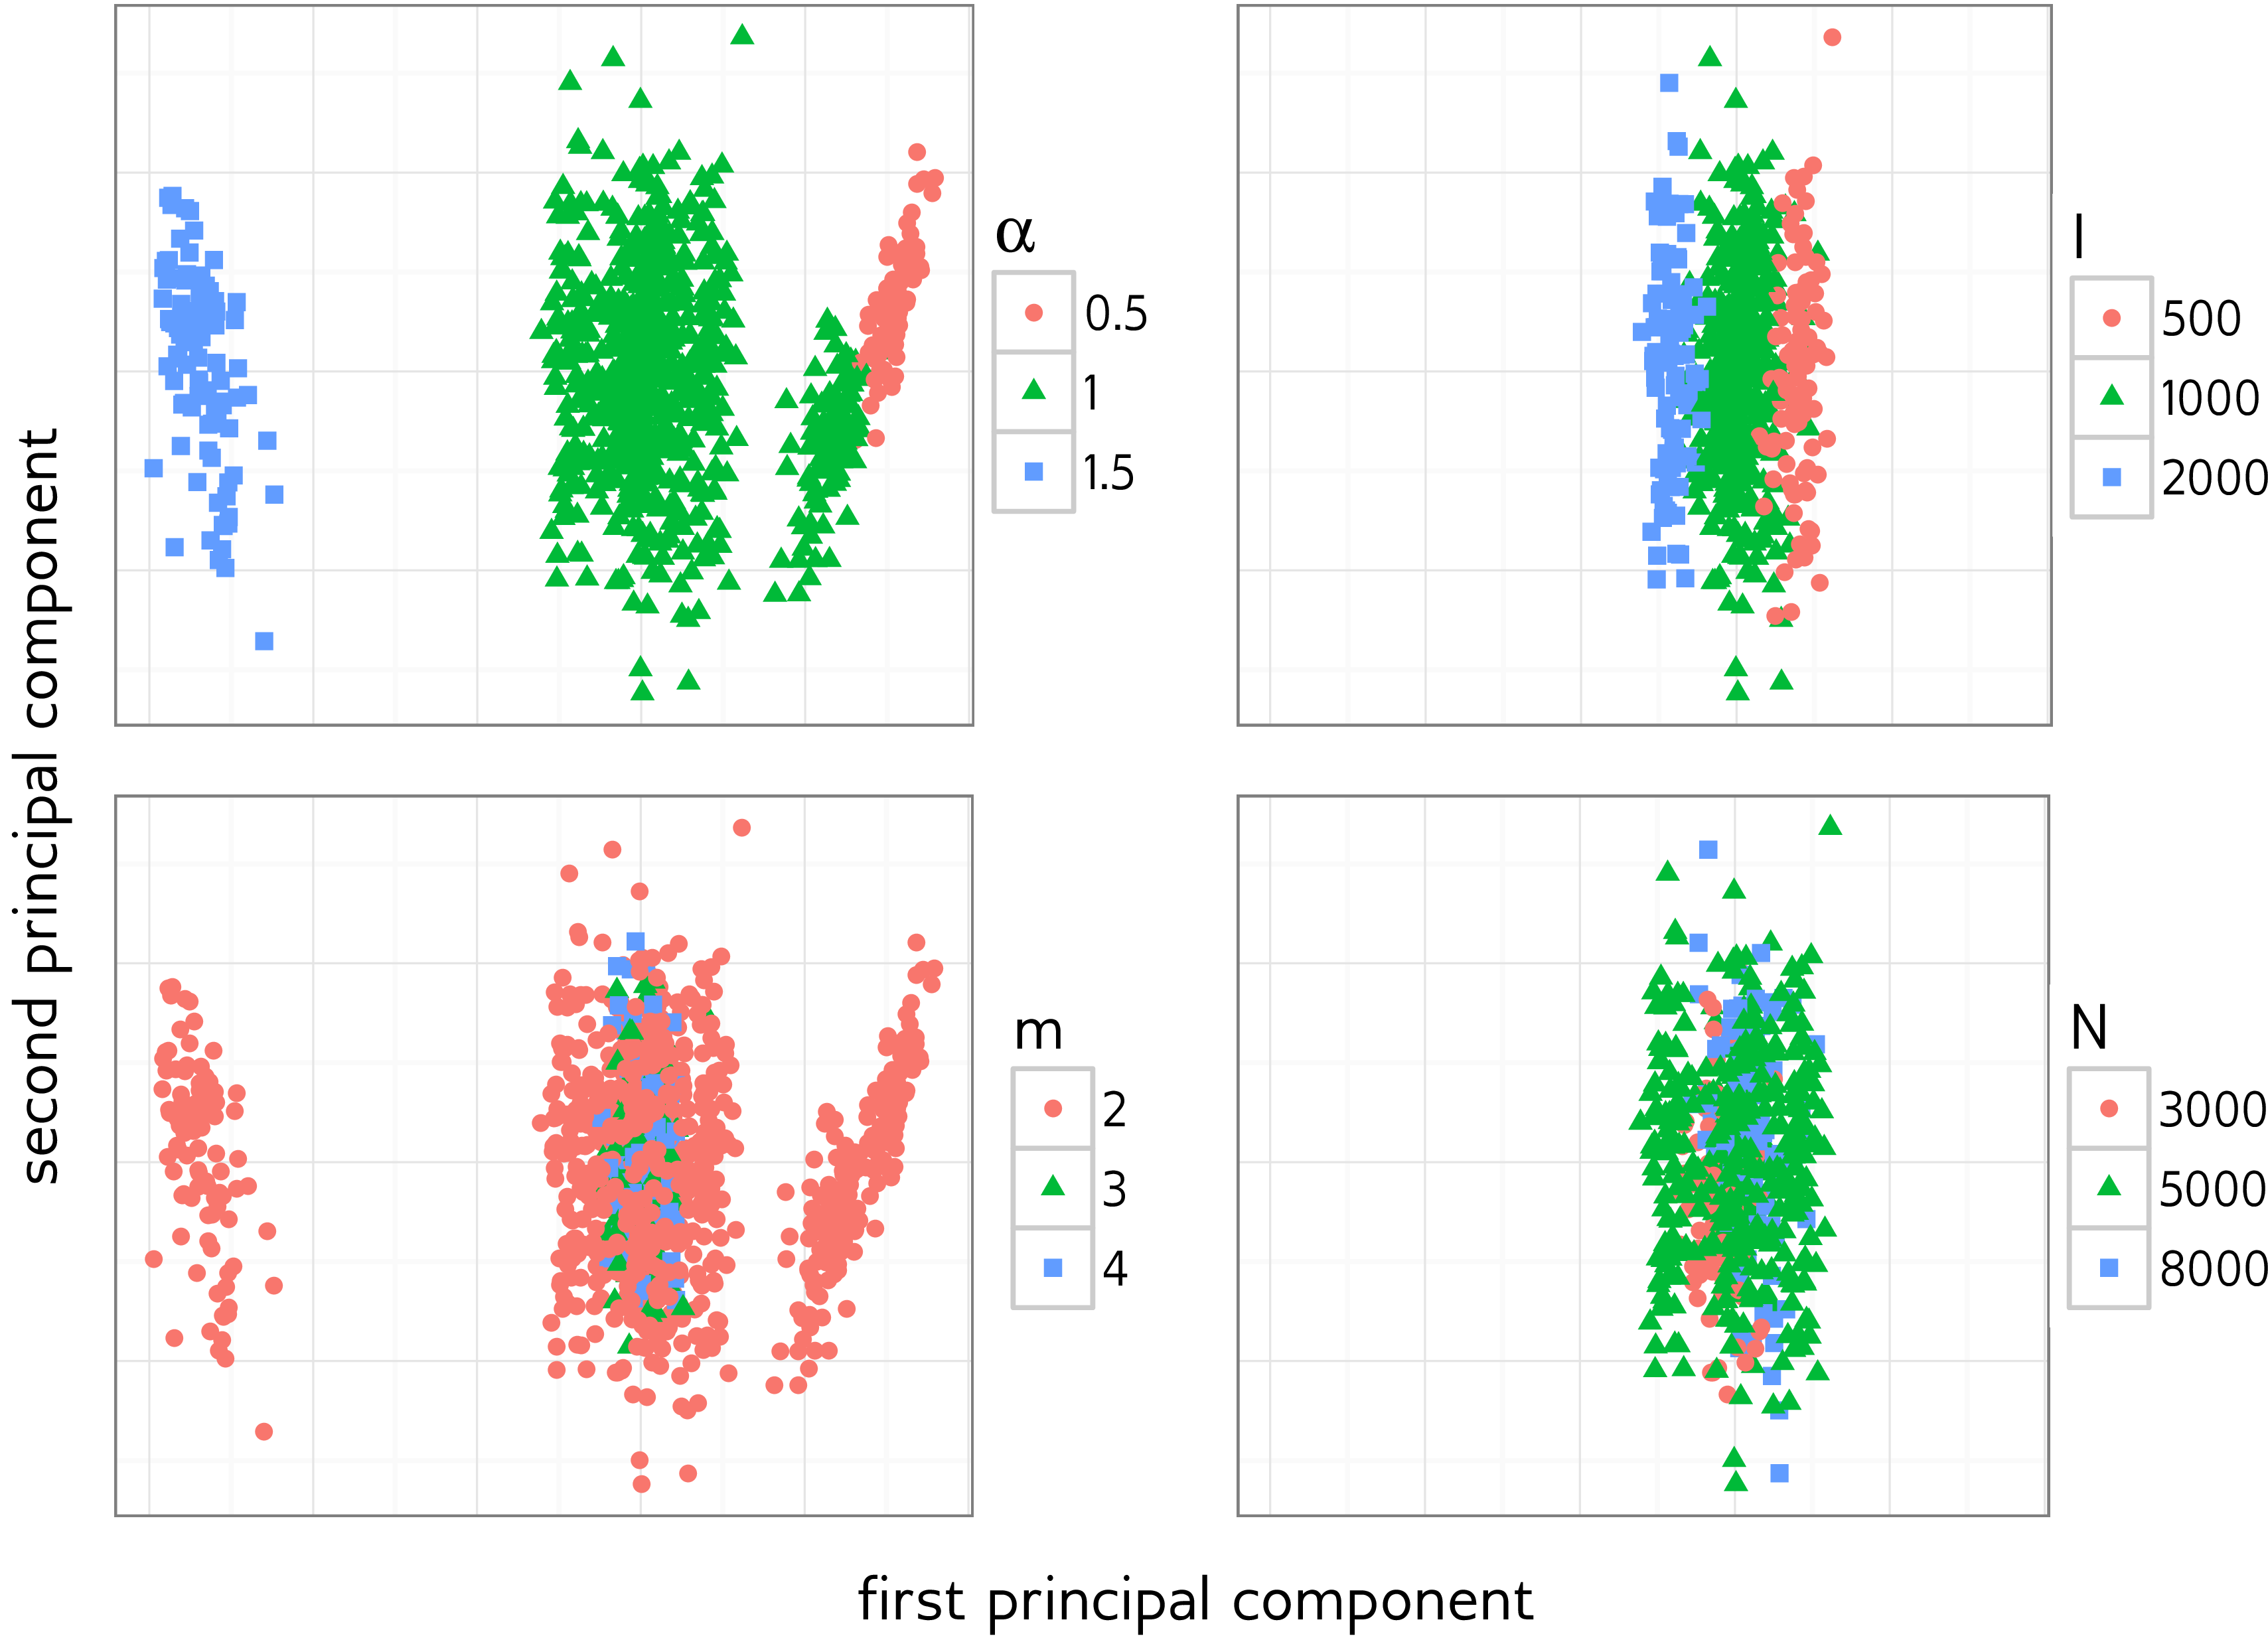
\includegraphics{kernel-kpca.pdf}
  \caption[Kernel-PCA projections of simulated trees under varying BA
           parameter values.]{
    Each parameter of the \gls{BA} model was individually varied to produce 300
    simulated trees. Kernel matrices were formed from all pairwise kernel
    scores among each set of 300 trees. The trees were projected onto the first
    two principal components of the kernel matrix calculated using \gls{kPCA}.
    All trees had 500 tips. The parameters not being varied were set to
    \gls{alpha} = 1, \gls{I} = 1000, \gls{m} = 2, and \gls{N} = 5000. The tree
    kernel meta-parameters were $\lambda = 0.3$ and $\sigma = 4$.
  }
  \label{fig:kpca}
\end{figure}



Accuracy of the \gls{kSVR} classifiers varied based on the parameter being
tested (\cref{fig:rsquared}, left). Classifiers based on two other tree
statistics, the \gls{nltt} and Sackin's index, generally exhibited worse
performance than the tree kernel, although the magnitude of the disparity
varied between the parameters (\cref{fig:rsquared}, centre and right). The
results were largely robust to variations in the tree kernel meta-parameters
$\lambda$ and $\sigma$, although accuracy varied between different epidemic and
sampling scenarios
(\cref{fig:alphacrossv,fig:mcrossv,fig:Icrossv,fig:Ncrossv}).

When classifying $\alpha$, the \gls{kSVR} classifier had an average $R^2$ of 
    0.92,
compared to 
    0.56
for the \gls{nltt}-based SVR, and
    0.75
for the linear regression against Sackin's index. There was little variation
about the mean for different tree and epidemic sizes. No classifier could
accurately identify the $m$ parameter in any epidemic scenario, with average
$R^2$ values of 
  0.12 for \gls{kSVR},
  0.01 for the \gls{nltt}, and
  0.06
for Sackin's index. Again, there was little variation in accuracy between
epidemic scenarios, although the accuracy of the \gls{kSVR} was slightly higher
on 1000-tip trees 
    (average $R^2$ 
     0.01,
     0.11,
     0.32
     for 100, 500, and 1000 tips respectively).

The accuracy of classifiers for $I$ varied significantly with the number of
tips in the tree. For 100-tip trees, the average $R^2$ values were
  0.7,
  0.55, and
  0.02
for the tree kernel, \gls{nltt}, and Sackin's index respectively. For 500-tip
trees, the values increased to
  0.93,
  0.83, and
  0.07.
Finally, the performance of classifiers for $N$ depended heavily on the
epidemic scenario. The $R^2$ of the \gls{kSVR} classifier ranged from
  0.08
for the smallest epidemic and smallest sample size, to
  0.82
for the largest. Likewise, $R^2$ for the \gls{nltt}-based SVR ranged from 
  0.01
to
  0.54.
Sackin's index did not accurately classify $N$ in any scenario, with an average
$R^2$ of
  0.03
and little variation between scenarios.

\begin{figure}[ht]
  \centering
  \includegraphics[width=\textwidth]{kernel-rsquared.pdf}
  \caption[Cross-validation accuracy of kernel-SVR, nLTT-based SVR, and
  Sackin's index regression classifiers for BA model parameters.]{
      Cross-validation accuracy of kernel-SVR classifier (left), SVR classifier
      using \gls{nltt} (centre), and linear regression using Sackin's index
      (right) for \gls{BA} model parameters. Kernel meta-parameters were set to
      $\lambda = 0.3$ and $\sigma = 4$. Each point was calculated based on 300
      simulated transmission trees over networks with three different values of
      the parameter being tested, assuming perfect knowledge of the other
      parameters. Vertical lines are empirical 95\% confidence intervals based
      on 1000 two-fold cross-validations. {\color{blue}\uline{ The classifiers
      for \gls{I} were not evaluated with 1000-tip trees, because one of the
      tested \gls{I} values was 500, and it is not possible to sample a tree of
      size 1000 from 500 infected individuals.}}
  }
  \label{fig:rsquared}
\end{figure}

\subsubsection*{Marginal parameter estimates with grid search}



{\color{red}\sout{The accuracy of grid search estimates largely paralleled that
of the \gls{kSVR} classifiers.}}\Cref{fig:gridest} shows point estimates and
{\color{blue}\uline{50\%}} and 95\% highest density intervals for each of the
\gls{BA} parameters, for one replicate experiment with 500-tip trees. Plots
showing the point estimates for all replicates can be found in
\cref{fig:gridptalpha,fig:gridptI,fig:gridptm,fig:gridptN}. For all parameters
except $m$, the error of point estimates was negatively correlated with the
number of sampled tips in the tree (for \gls{alpha}, \gls{I}, and \gls{N}
respectively: Spearman's $\rho$ = \ensuremath{-0.22},
\ensuremath{-0.51}, \ensuremath{-0.16}; $p$-values
    $4\!\times\!10^{-4}$,
    ${<}10^{-5}$,
    $0.01$).
The 95\% highest density intervals obtained for all parameters were extremely
wide, occupying $>$75\% of the grid in all cases (\cref{fig:gridest}).

{\color{blue}\uline{Across all replicates, $R^2$ values for the correlations
between the estimated and true values were
    $0.91$,
    $0.91$,
    $0.25$, and
    $0.54$
for \gls{alpha}, \gls{I}, \gls{m}, and \gls{N} respectively. The mean absolute
errors of the point estimates were
    $0.14$,
    $310$,
    $1.31$, and
    $2419$,
representing
    $7$\%,
    $8$\%,
    $26$\%, and
    $17$\%
of the respective grids.}

\uline{Qualitatively, each of the parameters exhibited weak identifiability
within particular sections of the grid} (\cref{fig:gridest}). \uline{The 50\%
\glspl{HDI} for \gls{alpha} were nearly identical for the values $\gls{alpha}
\leq 0.5$ (on average [X-X]) and for $\gls{alpha} \geq 1.5$ ([X-X]).
For \gls{I}, similar 50\% \gls{HPD} were observed for $\gls{I} \leq 1500$
(average [X-X]) and for $\gls{I} > 3000$ ([X-X]). For \gls{m}, both the 50\%
and 95\% \glspl{HDI} were generally identical for $\gls{m} > 2$ (average [X-X]
for 50\% and [X-X] for 95\% \gls{HDI}). We did not observe a similar pattern
for \gls{N}, however the boundaries of the \gls{HDI} did not always
monotonically increase with the actual value.}

\Cref{fig:gridalpha,fig:gridI,fig:gridm,fig:gridN} \uline{show kernel score
distributions of kernel scores along the grid for each parameter. The
distributions for some values, such as $\gls{alpha} = 1.25$, $\gls{I} = 500$
and $4500$, $\gls{m} = 1$, and $\gls{N} = 1000$, exhibited distinct peaks
around the true value. This indicates that these values produce distinctively
shaped trees that can be identified with the tree kernel, when the other
parameter values are fixed and known. However, for the majority of values of
each parameter, the score distributions were fairly flat around the true value. 
This means there is a range of values which produce similarly shaped trees, and
the parameter is less identifiable within that range. The exception was
\gls{I}, whose score distributions exhibited a more or less rounded shape with
the highest point near the true value. }}

{\color{red}\sout{The \gls{alpha} parameter was the most accurately estimated,
with point estimates having an average deviation of 
    0.14
from the true value, on a grid from 0 to 2. The error of point estimates varied
significantly between true values of \gls{alpha}
    (one-way \gls{ANOVA}, $p$ ${<}10^{-5}$). In
particular, errors were lower for the values \gls{alpha} = 1.0 and 1.25 than
for the other values
    (average errors 
    0.03
    for \gls{alpha} = 1.0 or 1.5 vs.
    0.17
    for \gls{alpha} $\neq$ 1.0 or 1.5),
and this difference was significant
    (Wilcoxon rank-sum test, $p {<}10^{-5}$,
}\cref{fig:gridptalpha}).
\sout{These two values exhibited different qualitative behaviour than the other
values in terms of the distribution of kernel scores along the grid
}(\cref{fig:gridalpha}). \sout{In particular, there was a pronounced peak in scores
around the true value, in contrast to the other values where the scores were
flat around the true value. The effect was most obvious for the value
\gls{alpha} = 1.25.}}

%The average absolute error of the point estimates for \gls{I} was 
%    d["I", round(mean(error))] individuals,
%on a grid of 500 to 5000, and these errors differed between true values of
%\gls{I}
%    (one-way \gls{ANOVA}, $p pp(av["I", p], eq=TRUE)$).
%The errors for $2000 \leq I \leq 3000$ were higher than those for the other
%values
%    (average errors
%     d["I", .SD[true_value >= 2000 & true_value <= 3000, round(mean(error))]]
%     for $2000 \leq I \leq 3000$ vs.
%     d["I", .SD[true_value < 2000 | true_value > 3000, round(mean(error))]]
%     for $I < 2000$ or $I > 3000$),
%and this difference was significant
%    (Wilcoxon rank-sum test, $p pp(I.test$p.value, eq=TRUE)$,
%     \cref{fig:gridptI}).
%Kernel score distributions for all test values exhibited a similar rounded
%shape (\cref{fig:gridI}). 
%
%The average error for \gls{m} was
%    d["m", round(mean(error), 2)] edges per vertex,
%on a grid from 1 to 6. The error varied significantly between the true values
%of \gls{m} 
%    (one-way \gls{ANOVA}, $p pp(av["m", p], eq=TRUE)$).
%Errors for the value \gls{m} = 1 were lower than the other values
%    (average errors
%    d["m", .SD[true_value == 1, round(mean(error), 2)]]
%    for $m = 1$ vs.
%    d["m", .SD[true_value > 1, round(mean(error), 2)]]
%    for $m > 1$),
%and this difference was significant
%    (Wilcoxon rank-sum test, $p pp(m.test$p.value, eq=TRUE)$,
%     \cref{fig:gridptm}).
%The value $m = 1$ causes the network to take on a distinct shape relative to
%higher \gls{m} values, namely a tree (\ie there are no cycles, see
%\cref{subsec:treeshape}). The kernel score distribution had a peak at $m = 1$
%when this was the true value, and a valley at $m = 1$ when the true value of
%$m$ was greater that 1 (\cref{fig:gridm}).
%
%The average error for \gls{N} was 
%    d[parameter == "N", round(mean(error))] individuals,
%on a grid from 1000 to 15000, and was varied significantly with the true value
%of \gls{N}
%    (one-way \gls{ANOVA}, $p pp(av["N", p], eq=TRUE)$).
%The errors were lower for $N \leq 3000$
%    (average errors
%     d["N", .SD[true_value <= 3000, round(mean(error))]]
%     for $N \leq 3000$ vs.
%     d["N", .SD[true_value > 3000, round(mean(error))]]
%     for $N > 3000$),
%and this difference was significant
%    (Wilcoxon rank-sum test, $p pp(N.test$p.value, eq=TRUE)$,
%     \cref{fig:gridptN}).
%The kernel score distribution had a peak at $N = 1000$ when this was the true
%value, and a valley there otherwise (\cref{fig:gridN}). Except for this valley,
%the distributions were flat for $N > 3000$.

\begin{figure}[ht]
  \centering
  \includegraphics[width=\textwidth]{gridsearch-example}
  \caption[
    Grid search estimates of \gls{BA} model parameters for one replicate
    experiment with trees of size 500.
  ]{
    Grid search estimates of \gls{BA} model parameters for one replicate
    experiment with trees of size 500. Point estimates (dots), 95\% highest
    density intervals (lines), and 50\% highest density intervals (notches) for
    each \gls{BA} model parameter, obtained using grid search. Networks and
    transmission trees were simulated over a grid of values for each parameter
    while holding the others fixed. For a subset of the grid values ($x$-axis),
    test networks and trees were created and compared to each tree on the grid
    using the tree kernel. The kernel scores along the grid were normalized to
    resemble a probability distribution, from which the mode and highest
    density interval were calculated. 
  } 
  \label{fig:gridest}
\end{figure}

\subsubsection*{Joint parameter estimates with \software{netabc}}



\Cref{fig:abcptm2} shows {\color{red}\sout{\gls{MAP}}}
{\color{blue}\uline{posterior mean}} point estimates of the BA model parameters
obtained with kernel-assisted ABC on simulated data. The estimates shown
correspond only to the simulations where the $m$ parameter was set to 2,
however the results for $m = 3$ and $m = 4$ were similar
(\cref{fig:abcptm3,fig:abcptm4}). Average boundaries of 95\% \gls{HPD}
intervals are given in \cref{tab:abchpd}.

{\color{blue}
\uline{Across all simulations, the median [\gls{IQR}] absolute errors of the parameter 
estimates obtained with \software{netabc} were
    0.11 
    [0.03 - 
    0.25]
for \gls{alpha},
    492 
    [294 - 
    782]
for \gls{I},
    1 
    [0 - 
    1]
for \gls{m}, and
    4153 
    [3660 - 
    4489]
for \gls{N}. These errors comprised, respectively,
    6\%,
    11\%,
    17\%, and
    29\%
of the regions of nonzero prior density. Average \gls{HPD} interval widths were
    0.68,
    2454,
    3.01, and
    12046,
representing 
    34\%,
    55\%,
    50\%, and
    83\%
of the nonzero prior density regions. Point estimates of \gls{I} were upwardly
biased: \gls{I} was overestimated in
    69
out of 
    72
simulations
    (96\%).
The estimates for \gls{m} and \gls{N} were similar across all simulations
(median [IQR] point estimates
    3
    [3 - 
    3]
and 
    9153
    [8660 - 
    9489])
regardless of the true values of any of the \gls{BA} parameters.}

\uline{To analyse the effects of the true parameter values on the
accuracy our estimates of \gls{alpha} and \gls{I}, we fitted one \glspl{GLM}
for each of these two parameters, with error rate as the dependent variable and
the true parameter values as independent variables. Since the estimates of
\gls{m} and \gls{N} were roughly equal across all simulations}
(\cref{fig:abcptm2,fig:abcptm3,fig:abcptm4}), \uline{\glspl{GLM} were not
fitted for these parameters. The estimated coefficients are shown in
}\cref{tab:glmalpha,tab:glmI}. \uline{For the parameters \gls{alpha}, \gls{I},
and \gls{N}, the \gls{GLM} were fitted using the inverse link function. That
is, if $p$ is the true value of the parameter and $\hat{p}$ is a random
variable representing our estimate of the parameter, the \gls{GLM} posits a
relationship of the form }
\[
    \E(|p-\hat{p}|) = (\beta_0 + \beta_\alpha \alpha + \beta_I I + \beta_m m)^{-1},
\]
\uline{where the $\beta$'s are coefficients to be fitted. If the true value
\gls{alpha}, say, is increased by one, the \emph{inverse} of the expected
absolute error will increase by $\beta_\alpha$. If $\beta_\alpha$ is positive,
it means that the absolute error decreases as the true value of \gls{alpha}
increases.}}



% latex table generated in R 3.2.3 by xtable 1.8-2 package
% Thu Jun  9 16:06:29 2016
\begin{table}[ht]
\centering
\begin{tabular}{llll}
  \hline
Parameter & Estimate & Standard error & $p$-value \\ 
  \hline
(Intercept) & $2$ & $0.6$ & $0.01$ \\ 
  $\alpha$ & $10$ & $2$ & ${<}10^{-5}$ \\ 
  I & $-3\!\times\!10^{-4}$ & $2\!\times\!10^{-4}$ & $0.7$ \\ 
  m & $0.5$ & $0.2$ & $0.01$ \\ 
   \hline
\end{tabular}
\caption[Parameters of a fitted GLM relating error in estimated $\alpha$ to true values of BA parameters.]{Parameters of a fitted GLM relating error in estimated $\alpha$ to true values of BA parameters. GLM was fitted with a Gaussian distribution and inverse link function. Coefficients are interpretable as additive effects on the inverse of the mean error.} 
\label{tab:glmalpha}
\end{table}
% latex table generated in R 3.2.3 by xtable 1.8-2 package
% Thu Jun  9 16:06:29 2016
\begin{table}[ht]
\centering
\begin{tabular}{llll}
  \hline
Parameter & Estimate & Standard error & $p$-value \\ 
  \hline
(Intercept) & $0.004$ & $5\!\times\!10^{-4}$ & ${<}10^{-5}$ \\ 
  $\alpha$ & $-0.001$ & $2\!\times\!10^{-4}$ & ${<}10^{-5}$ \\ 
  I & $-4\!\times\!10^{-7}$ & $2\!\times\!10^{-7}$ & $0.05$ \\ 
  m & $-7\!\times\!10^{-5}$ & $8\!\times\!10^{-5}$ & $1$ \\ 
   \hline
\end{tabular}
\caption[Parameters of a fitted GLM relating error in estimated $I$ to true values of BA parameters.]{Parameters of a fitted GLM relating error in estimated $I$ to true values of BA parameters. GLM was fitted with a gaussian distribution and inverse link function. Coefficients are interpretable as additive effects on the inverse of the mean error.} 
\label{tab:glmI}
\end{table}


{\color{blue}\uline{The \gls{GLM} analysis indicated that the error in estimates of
\gls{alpha} decreased with larger true values of \gls{alpha} 
    ($p {<}10^{-5}$)
and \gls{m}
    ($p =0.01$)
but was not significatly affected by \gls{I}} (\cref{tab:glmalpha}). 
\uline{Qualitatively, \gls{alpha} seemed to be only weakly identifiable between
the values of 0 and 0.5} (\cref{fig:abcptm2}). \uline{The error in the
estimated prevalence \gls{I} was slightly lower for smaller values of
\gls{alpha}
    ($p {<}10^{-5}$)
and \gls{I}
    ($p =0.05$),
but was not significantly affected by the true value of \gls{m}} 
(\cref{tab:glmI}).}

{\color{red}\sout{
The accuracy of the parameter estimates obtained with kernel-assisted ABC
paralleled the results from the \gls{kSVR} classifier. Of the four parameters,
$\alpha$ was the most accurately estimated, with point estimates having a
median [IQR] absolute error of 
    0.11 
    [0.03 - 
    0.25].
The errors when the true value of $\alpha$ was zero were significantly greater
than those for the other values 
    (Wilcoxon rank-sum test, $p$ = $0$).
Errors in estimating $\alpha$ 
%also varied with the true value of $m$ just at
%the threshold of statistical significance
%    (one-way ANOVA, $p 
%    pp(anova(lm(alpha_error~true_m, d))[1, "Pr(>F)"], eq=TRUE)$),
did not vary across the true values of $m$ or $I$ (both
one-way ANOVA).}

\sout{Estimates for $I$ were relatively accurate, with point estimate errors of
    492 
    [294 - 
    782] individuals.
These errors were significantly higher when the true value of $\alpha$ was
at least 1
    (Wilcoxon rank-sum test, $p$ = $0$)
and when the true value of $I$ was 2000 ($p < 10^{-5}$). The true value of $m$
did not affect the estimates of $I$ (one-way ANOVA).}

\sout{The $m$ parameter was estimated correctly in
    37 \%
of simulations barely better than random guessing. The true values of the other
parameters did not significantly affect the
estimates of $m$ (both one-way ANOVA).}

\sout{Finally, the total number of nodes $N$ was consistently over-estimated by about
a factor of two (error 4153
[3660 - 4489] individuals). No parameters influenced the accuracy of the $N$
estimates (all one-way ANOVA).}}

\begin{figure}[ht]
  \centering
  \includegraphics[width=\textwidth]{abc-point-estimate-m2}
  \vspace{6pt}
  \caption[
    Posterior mean point estimates for \gls{BA} model parameters obtained by
    running \software{netabc} on simulated data, for simulations with \gls{m} =
    2.
  ]{
    Posterior mean point estimates for \gls{BA} model parameters obtained by
    running \software{netabc} on simulated data, for simulations with \gls{m} =
    2. Dashed lines indicate true values. (A) Estimates of \gls{alpha} and
    \gls{I} which were varied in these simulations against known values. (B)
    Estimates of \gls{m} and \gls{N} which were held fixed in these simulations
    at the values \gls{m} = 2 and \gls{N} = 5000.
  }
  \label{fig:abcptm2}
\end{figure}

\begin{table*}[ht]
  \centering
  % latex table generated in R 3.2.3 by xtable 1.8-2 package
% Fri Jun 17 12:51:45 2016
\begin{tabular}{lr>{\raggedleft\arraybackslash}p{2.5cm}>{\raggedleft\arraybackslash}p{2.5cm}>{\raggedleft\arraybackslash}p{2.5cm}}
  \hline
Parameter & True value & Mean point estimate & Mean HPD lower bound & Mean HPD upper bound \\ 
  \hline
$\alpha$ & 0.0 & 0.36 & 0.01 & 0.81 \\ 
   & 0.5 & 0.43 & 0.04 & 0.83 \\ 
   & 1.0 & 0.90 & 0.51 & 1.09 \\ 
   & 1.5 & 1.52 & 1.26 & 1.81 \\ 
  $I$ & 1000 & 1450 & 651 & 2592 \\ 
   & 2000 & 2622 & 1114 & 4080 \\ 
  $m$ & 2 & 2.96 & 2.00 & 5.00 \\ 
   & 3 & 3.04 & 2.04 & 4.96 \\ 
   & 4 & 3.17 & 1.88 & 5.00 \\ 
  $N$ & 5000 & 9041 & 2613 & 14659 \\ 
   \hline
\end{tabular}

  \caption[
      Average posterior mean point estimates and 95\% highest posterior density
      (HPD) interval widths for BA model parameter estimates obtained with
      kernel-assisted ABC.
  ]{
      Average posterior mean point estimates and 95\% highest posterior density
      (HPD) interval widths for BA model parameter estimates obtained with
      kernel-assisted ABC. Three transmission trees were simulated under each
      combination of the listed parameter values, and the parameters were
      estimated with kernel-assisted ABC without training.
  }
  \label{tab:abchpd}
\end{table*}



The dispersion of the ABC approximation to the posterior also varied between
the parameters, with narrower HPD intervals for the parameters with more
accurate point estimates (\cref{tab:abchpd}). \Cref{fig:abcex} shows
the distributions for one simulation. Equivalent plots for one replicate
simulation with each studied parameter combination can be found in
\cref{fig:0.0-1000-2-5000-0,fig:0.5-1000-2-5000-0,fig:1.0-1000-2-5000-0,fig:1.5-1000-2-5000-0,fig:0.0-2000-2-5000-0,fig:0.5-2000-2-5000-0,fig:1.0-2000-2-5000-0,fig:1.5-2000-2-5000-0,fig:0.0-1000-3-5000-0,fig:0.5-1000-3-5000-0,fig:1.0-1000-3-5000-0,fig:1.5-1000-3-5000-0,fig:0.0-2000-3-5000-0,fig:0.5-2000-3-5000-0,fig:1.0-2000-3-5000-0,fig:1.5-2000-3-5000-0,fig:0.0-1000-4-5000-0,fig:0.5-1000-4-5000-0,fig:1.0-1000-4-5000-0,fig:1.5-1000-4-5000-0,fig:0.0-2000-4-5000-0,fig:0.5-2000-4-5000-0,fig:1.0-2000-4-5000-0,fig:1.5-2000-4-5000-0}. HPD intervals around $\alpha$ and $I$ were often narrow
relative to the region of nonzero prior density, whereas the intervals for $m$
and $N$ were more widely dispersed.

\begin{figure}[ht]
    \centering
    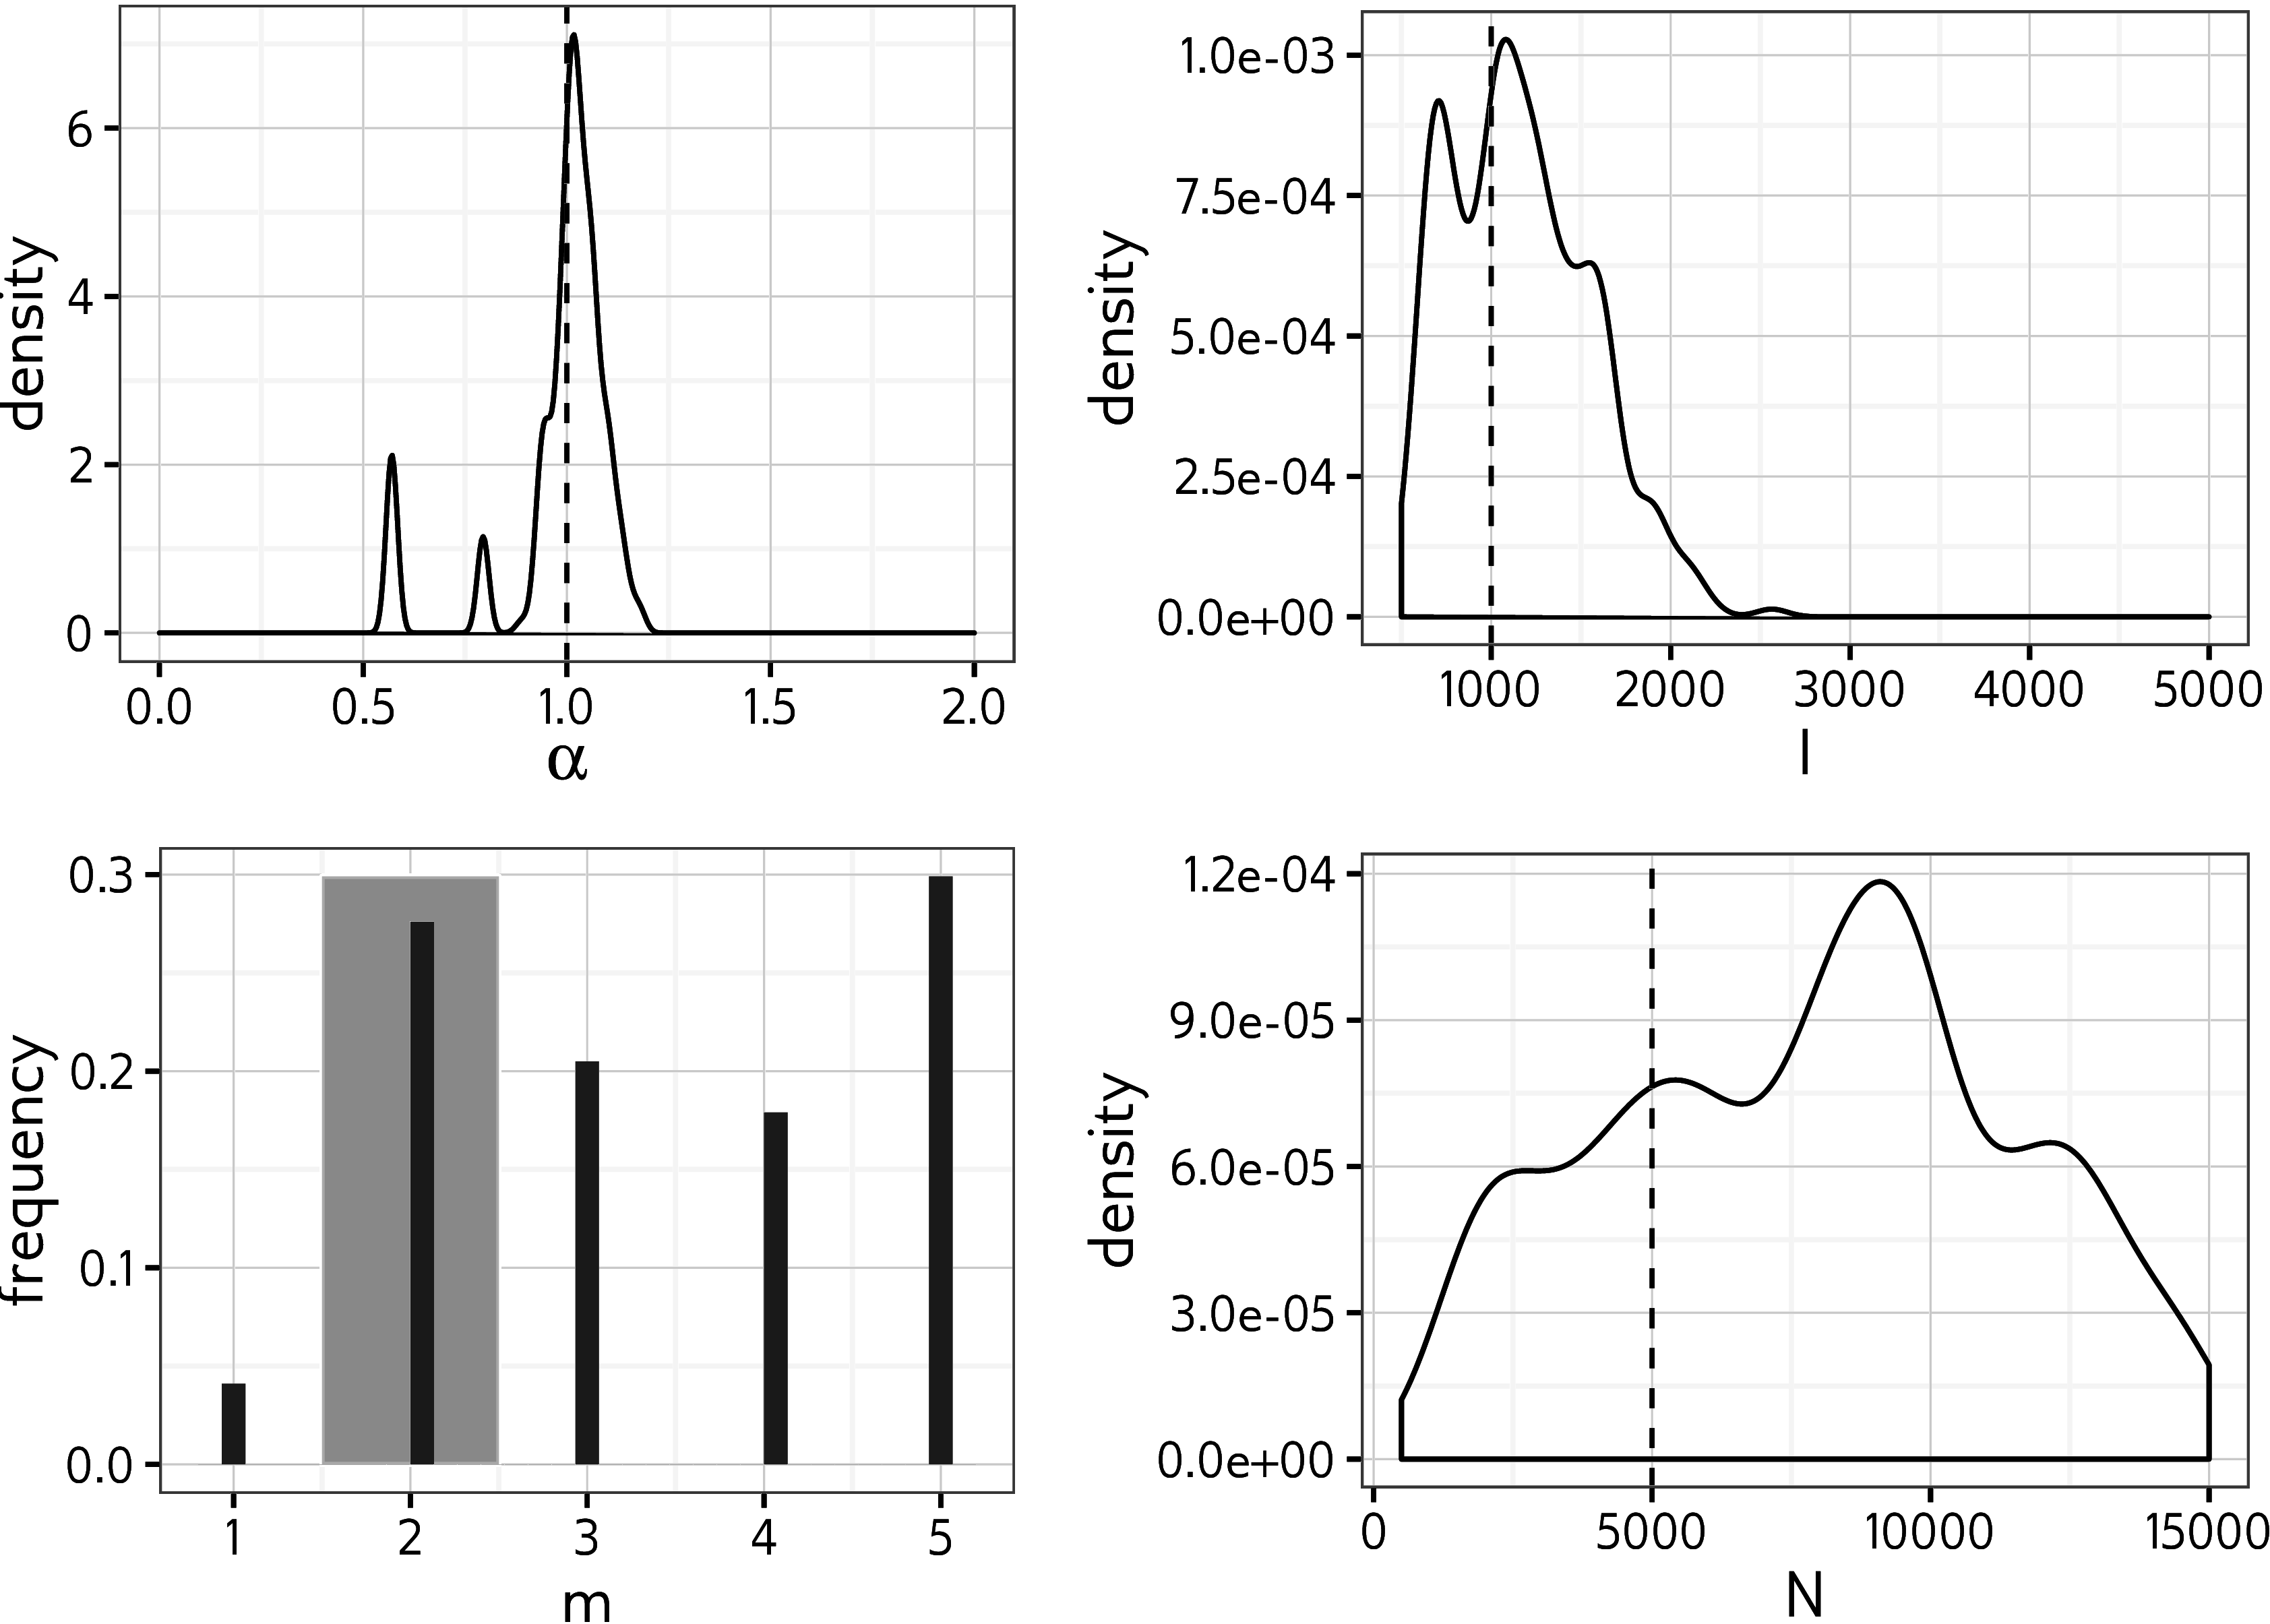
\includegraphics[width=\textwidth]{abc-posterior-example}
  \vspace{6pt}
  \caption[
    Marginal posterior distributions of BA model parameters estimated
    with kernel-assisted ABC for a single simulated transmission tree.
  ]{
    Marginal posterior distributions of BA model parameters estimated
    with kernel-assisted ABC for a single simulated transmission tree. Dotted
    lines indicate true values, solid lines indicate posterior mean point
    estimates, and shaded areas show 95\% highest posterior density intervals.
  }
  \label{fig:abcex}
\end{figure}



To test the effect of model misspecification, we simulated one network where
the nodes exhibited heterogeneous preferential attachment power (half 0.5, the
other half 1.5), with $m$ = 2, $N$ = 5000, and $I$ = 1000. The posterior mean
[95\% HPD] estimates for each parameter were: 
$\alpha$, 
  1.03 
  [0.67 -
   1.18];
$I$,
  1474 
  [511 -
   2990];
$m$,
  3 
  [1 -
   5];
$N$,
  9861 
  [3710-
   14977].
The approximate posterior distributions for this simulation are shown in
\cref{fig:mixed}. To test the effect of sampling bias, we sampled one
transmission tree in a peer-driven fashion, where the probability to sample a
node was twice as high if one of its peers had already been sampled. The
parameters for this experiment were $N$ = 5000, $m$ = 2, $\alpha$ = 0.5, and
$I$ = 2000. The estimated values were
$\alpha$, 
  0.3 
  [0 -
   0.63];
$I$,
  2449 
  [1417 -
   3811];
$m$,
  3 
  [2 -
   5];
$N$,
  9132 
  [2852 -
   14780].
The approximate posterior distributions are shown in \cref{fig:peerdriven}. Both
of these results were in line with estimates obtained on other simulated
datasets (\cref{tab:abchpd}), although the estimate of peer-driven sampling for
$\alpha$ was somewhat lower than typical.

%<<abc_glm, include=FALSE>>=
%    source("global.R")
%    options(scipen=-1, digits=2)
%@
%
%<<alpha_glm, include=FALSE>>=
%    # alpha_error is influenced by alpha and m but not I
%    stopifnot(alpha.glm[Parameter == "alpha", min(p) < 0.05])
%    stopifnot(alpha.glm[Parameter == "m", min(p) < 0.05])
%    stopifnot(alpha.glm[Parameter == "I", min(p) > 0.05])
%
%    # alpha_error is correlated with true_alpha
%    alpha.test <- d[,cor.test(alpha_error, true_alpha, method="spearman")]
%    stopifnot(alpha.test$p.value < 0.05)
%
%    # alpha_error is not correlated with true_m
%    alpha.m.cor <- d[,cor.test(alpha_error, true_m)]
%    stopifnot(alpha.m.cor$p.value < 0.05)
%@
%
%We used \software{netabc} to estimate the parameters of the \gls{BA} model on
%simulated trees where the true parameter values were known. Point estimates for
%each parameter are shown in \cref{fig:abcptm2} for the simulations with \gls{m} =
%2. The results for the other values of \gls{m} were similar
%(\cref{fig:abcptm3,fig:abcptm4}). The median [IQR] absolute error of estimates
%of \gls{alpha} across all simulations was
%    d[,median(alpha_error)] 
%    [d[,quantile(alpha_error, 0.25)]-d[,quantile(alpha_error, 0.75)]].
%\Gls{GLM} analysis indicated that the true values of both \gls{alpha} and
%\gls{m} had significant effects on the error in estimated \gls{alpha}
%    ($p$ values $pp(alpha.glm[Parameter == "alpha", min(p)], eq=FALSE)$
%     $pp(alpha.glm[Parameter == "m", min(p)], eq=FALSE)$,
%     \cref{tab:glmalpha}),
%but the true value of \gls{I} did not. There was a significant negative
%correlation between the true value of \gls{alpha} and the error
%    (Spearman's $\rho$ = round(alpha.test$estimate, 2),
%     $p pp(alpha.test$p.value, eq=TRUE)$).
%There was a negative correlation between \gls{m} and the error in \gls{alpha}
%    (Spearman's $\rho$ = round(alpha.m.cor$estimate, 2),
%    $p pp(alpha.m.cor$p.value, eq=FALSE)$).
%
%<<I_glm, include=FALSE>>=
%    # I_error is influenced by alpha and I but not by m
%    stopifnot(I.glm[Parameter == "alpha", min(p) < 0.05])
%    stopifnot(I.glm[Parameter == "m", min(p) > 0.05])
%    stopifnot(I.glm[Parameter == "I", min(p) < 0.05])
%
%    # correlation between I_error and true_alpha
%    I.alpha.cor <- d[,cor.test(I_error, true_alpha, method="spearman")]
%    stopifnot(I.alpha.cor$p.value < 0.05)
%
%    # correlation between I_error and true_I
%    I.I.cor <- d[,cor.test(I_error, true_I, method="spearman")]
%    stopifnot(I.alpha.cor$p.value < 0.05)
%@
%
%The mean error in the estimated value of \gls{I} was
%    d[,round(median(I_error))] 
%    [d[,round(quantile(I_error, 0.25))]-d[,round(quantile(I_error, 0.75))]],
%an over-estimate of roughly a factor of 1.5
%(\cref{fig:abcptm2,fig:abcptm1,fig:abcptm3,fig:abcptm4}). \Gls{GLM} analysis
%indicated a relationship between the error in estimated \gls{I}, and the true
%values of \gls{alpha} and \gls{I}
%    ($p$ values $pp(I.glm[Parameter == "alpha", min(p)], eq=FALSE)$
%     $pp(alpha.glm[Parameter == "I", min(p)], eq=FALSE)$,
%     \cref{tab:glmalpha}),
%but not the true value of \gls{m}. There was a significant correlation between 
%the true value of \gls{alpha} and the error in estimated \gls{I}
%    (Spearman's $\rho$ = I.alpha.cor$estimate,
%     $p pp(I.alpha.cor$p.value, eq=TRUE)$),
%and between the true value of \gls{I} and the error in estimated \gls{I}
%    (Spearman's $\rho$ = I.I.cor$estimate,
%     $p pp(I.I.cor$p.value, eq=TRUE)$).
%
%<<m_glm, include=FALSE>>=
%    # effects of parameters on m_error
%    stopifnot(m.glm[Parameter == "m", min(p)] < 0.05)
%    stopifnot(m.glm[Parameter == "alpha", min(p)] > 0.05)
%    stopifnot(m.glm[Parameter == "I", min(p)] > 0.05)
%
%    # m was only estimated correctly in just over 20\% of simulations with m > 2
%    m.tbl <- prop.table(table(d[true_m > 1,m_error]))
%    stopifnot(m.tbl[1] > 0.2 & m.tbl[1] < 0.3)
%
%    # with m = 1, over 95% of simulations are right
%    m1.est <- d[true_m == 1, m_error]
%    stopifnot(sum(m1.est == 0) / length(m1.est) > 0.95)
%    stopifnot(sum(m1.est == 0) / length(m1.est) < 1)
%@
%
%\gls{GLM} analysis showed an effect of the true value of \gls{m} on the error
%in the estimated \gls{m}
%    ($p pp(m.glm[Parameter == "m", min(p)])$,
%     \cref{tab:glmm}).
%When the true value of \gls{m} was 1, the correct value was recovered by
%\software{netabc} in virtually every case
%    (sum(m1.est == 0) out of length(m1.est) simulations).
%However, when the true value of \gls{m} was 2 or higher, the correct value was
%recovered in only 
%    as.integer(m.tbl[1] * 100)\%
%of simulations, little better than random guessing. The \gls{GLM} analysis did
%not indicate any effects of the true parameter values on the error in estimated
%\gls{m} (\cref{tab:glmm}).
%
%<<N_glm, include=FALSE>>=
%    # alpha_error is influenced by alpha and m but not I
%    stopifnot(N.glm[Parameter == "alpha", min(p) < 0.05])
%    stopifnot(N.glm[Parameter == "I", min(p) < 0.05])
%    stopifnot(N.glm[Parameter == "m", min(p) > 0.05])
%
%    N.alpha.test <- d[,wilcox.test(.SD[true_alpha == 1.5, N_error], 
%                                   .SD[true_alpha < 1.5, N_error])]
%    stopifnot(N.alpha.test$p.value < 0.05)
%    N.I.test <- d[,wilcox.test(.SD[true_I == 3000, N_error], 
%                               .SD[true_I < 3000, N_error])]
%    stopifnot(N.I.test$p.value < 0.05)
%@
%
%Finally, the total number of nodes \gls{N} was consistently over-estimated by
%about a factor of two
%    (error d[,format(median(N_error), scientific=FALSE)] 
%    [d[,format(quantile(N_error, 0.25), scientific=FALSE)] - 
%     d[,format(quantile(N_error, 0.75), scientific=FALSE)]]).
%The fitted \gls{GLM} indicated that the true values of both \gls{alpha} and
%\gls{I} had an effect on the error in the estimated \gls{N}
%    ($p$-values $pp(N.glm[Parameter == "alpha", min(p)], eq=FALSE)$ and 
%     $pp(N.glm[Parameter == "I", min(p)], eq=FALSE)$,
%     \cref{tab:glmN}),
%but that the true value of \gls{m} did not. The error in the estimated \gls{N}
%when \gls{alpha} was equal to 1.5 was slightly lower than for other values of
%\gls{alpha}
%    (median [IQR] error rates 
%     d[true_alpha == 1.5, format(median(N_error), scientific=FALSE)] 
%    [d[true_alpha == 1.5, format(quantile(N_error, 0.25), scientific=FALSE)] - 
%     d[true_alpha == 1.5, format(quantile(N_error, 0.75), scientific=FALSE)]]
%     for \gls{alpha} = 1.5 vs. 
%     d[true_alpha < 1.5, format(median(N_error), scientific=FALSE)] 
%    [d[true_alpha < 1.5, format(quantile(N_error, 0.25), scientific=FALSE)] - 
%     d[true_alpha < 1.5, format(quantile(N_error, 0.75), scientific=FALSE)]]
%     for \gls{alpha} < 1.5),
%and this difference was statistically significant
%    (Wilcoxon rank-sum test, $p pp(N.alpha.test$p.value, eq=TRUE)$).
%Similarly, the error in the estimated \gls{N} when \gls{I} was equal to 3000 was
%lower than for other values of \gls{I}
%    (median [IQR] error rates 
%     d[true_I == 3000, format(median(N_error), scientific=FALSE)] 
%    [d[true_I == 3000, format(quantile(N_error, 0.25), scientific=FALSE)] - 
%     d[true_I == 3000, format(quantile(N_error, 0.75), scientific=FALSE)]]
%     for \gls{I} = 3000 vs. 
%     d[true_alpha < 3000, format(median(N_error), scientific=FALSE)] 
%    [d[true_alpha < 3000, format(quantile(N_error, 0.25), scientific=FALSE)] - 
%     d[true_alpha < 3000, format(quantile(N_error, 0.75), scientific=FALSE)]]
%     for \gls{I} < 3000),
%and this difference was statistically significant
%    (Wilcoxon rank-sum test, $p pp(N.I.test$p.value, eq=TRUE)$).
%
%\begin{figure}
%  \includegraphics{abc-point-estimate-m2}
%  \caption[\Acrlong{MAP} point estimates for \gls{BA} model parameters obtained
%    by running \software{netabc} on simulated data, for simulations with $m = 2$.] 
%  {
%    \Acrlong{MAP} point estimates for \gls{BA} model parameters obtained by         
%    running \software{netabc} on simulated data. Values shown are for               
%    simulations with \gls{m} = 2. Dashed lines indicate true values. (A)            
%    Estimates of \gls{alpha} and \gls{I} which were varied in these simulations  
%    against known values. (B) Estimates of \gls{m} and \gls{N} which were held   
%    fixed in these simulations at the values \gls{m} = 2 and \gls{N} = 5000. 
%  }
%  \label{fig:abcptm2}
%\end{figure}
%
%<<posterior_sims, echo=FALSE>>=
%    N <- 5000
%    replicate <- 0
%    lab <- NULL
%    for (m in c(2, 3, 4)) {
%    for (I in c(1000, 2000)) {
%    for (alpha in c(0, 0.5, 1, 1.5)) {
%        lab <- c(lab, sprintf("fig:%.1f-%d-%d-%d-%d", alpha, I, m, N, replicate))
%    }
%    }
%    }
%    lab <- paste(lab, collapse=",")
%@
%
%\Cref{fig:abcex} shows the \gls{ABC} approximation to the posterior
%distribution on the \gls{BA} parameters for one simulation. Equivalent plots
%for one replicate simulation with each combination of parameters can be found
%in \cref{lab}. \Gls{HPD} intervals around \gls{alpha} and \gls{I} were
%narrow relative to the region of nonzero prior density, whereas the intervals
%for $m$ and \gls{N} were widely dispersed. \Cref{tab:abchpd} shows point
%estimates and 95\% \gls{HPD} intervals averaged over all simulations.
%
%\begin{figure}
%  \includegraphics{{abc-posterior/1.0_1000_2_5000_0}.pdf}
%  \caption[Approximate marginal posterior distributions of BA model parameters
%      obtained by applying \textit{netabc} to a simulated transmission tree
%      with values $\alpha$ = 1.0, $I$ = 1000, $m$ = 2, and $N$ = 5000.]
%    {
%        Approximate marginal posterior distributions of BA model parameters
%        obtained by applying \textit{netabc} to a simulated transmission tree
%        with BA parameter values $\alpha$ = 1.0, $I$ = 1000, $m$ = 2, and $N$ =
%        5000. Vertical dashed lines indicate true values. Shaded areas are 95\%
%        highest posterior density intervals. $x$-axes indicate regions of
%        nonzero prior density.
%    }
%  \label{fig:abcex}
%\end{figure}
%
%
%\begin{table}
%    \centering
%    % latex table generated in R 3.2.3 by xtable 1.8-2 package
% Fri Jun 17 12:51:45 2016
\begin{tabular}{lr>{\raggedleft\arraybackslash}p{2.5cm}>{\raggedleft\arraybackslash}p{2.5cm}>{\raggedleft\arraybackslash}p{2.5cm}}
  \hline
Parameter & True value & Mean point estimate & Mean HPD lower bound & Mean HPD upper bound \\ 
  \hline
$\alpha$ & 0.0 & 0.36 & 0.01 & 0.81 \\ 
   & 0.5 & 0.43 & 0.04 & 0.83 \\ 
   & 1.0 & 0.90 & 0.51 & 1.09 \\ 
   & 1.5 & 1.52 & 1.26 & 1.81 \\ 
  $I$ & 1000 & 1450 & 651 & 2592 \\ 
   & 2000 & 2622 & 1114 & 4080 \\ 
  $m$ & 2 & 2.96 & 2.00 & 5.00 \\ 
   & 3 & 3.04 & 2.04 & 4.96 \\ 
   & 4 & 3.17 & 1.88 & 5.00 \\ 
  $N$ & 5000 & 9041 & 2613 & 14659 \\ 
   \hline
\end{tabular}

%    \caption[
%        Maximum \textit{a priori} estimates and 95\% highest posterior density
%        (HPD) interval boundaries for \gls{BA} model parameters estimated with
%        \software{netabc}, averaged over simulated transmission trees.
%    ]
%    {
%        Maximum \textit{a priori} estimates and 95\% highest posterior density
%        (HPD) interval boundaries for \gls{BA} model parameters estimated with
%        \software{netabc}, averaged over simulated transmission trees.
%    }
%    \label{tab:abchpd}
%\end{table}
%
%\subsubsection*{Effect of parameters on power-law exponent}
%
%\Cref{tab:glm} shows the estimated parameters for a log-link \gls{GLM} fitted
%to the observed distribution of \gls{gamma} values. The coefficients are
%interpretable as multiplicative effects.
%
%\begin{table}
%    \centering
%    % latex table generated in R 3.2.3 by xtable 1.8-2 package
% Tue Mar 15 09:15:55 2016
\begin{tabular}{rrrl}
  \hline
 & exp(Estimate) & Standard error & P-value \\ 
  \hline
(Intercept) & 1.63 & $5.1 \times 10^{-3}$ & $<10^{-5}$ \\ 
  $\alpha$ & 1.77 & $4.4 \times 10^{-3}$ & $<10^{-5}$ \\ 
  $m$ & 1.03 & $1.0 \times 10^{-3}$ & $<10^{-5}$ \\ 
  $N$ & 1.00 & $5.8 \times 10^{-7}$ & $<10^{-5}$ \\ 
  $\alpha \times m$ & 1.00 & $8.7 \times 10^{-4}$ & $<10^{-5}$ \\ 
  $\alpha \times N$ & 1.00 & $5.0 \times 10^{-7}$ & $<10^{-5}$ \\ 
  $m \times N$ & 1.00 & $1.1 \times 10^{-7}$ & $<10^{-5}$ \\ 
  $\alpha \times m \times N$ & 1.00 & $9.9 \times 10^{-8}$ & $<10^{-5}$ \\ 
   \hline
\end{tabular}

%    \caption{Estimated \gls{GLM} parameters for relationship between power-law
%    exponent \gls{gamma} and \gls{BA} model parameters.}
%    \label{tab:glm}
%\end{table}


\section{Application to real world HIV data}
\label{sec:hiv}

\subsection{Methods}

{\color{blue}\uline{
The synthetic data experiments presented in the previous section demonstrated 
that the \gls{alpha} and \gls{I} parameters, and to a lesser extent the \gls{N}
parameter, had measurable impacts on tree shape and were identifiable with
kernel-assisted \gls{ABC}. Therefore, our next step was to use
\software{netabc} to estimate the parameters of the \gls{BA} model for real
world \gls{HIV} epidemics. }} Because the \gls{BA} model assumes a single
connected contact network, it is most appropriate to apply to groups of
individuals who are epidemiologically related. Therefore, we searched for
published \gls{HIV} datasets which originated from existing clusters, either
phylogenetically or geographically defined. In addition, we analysed an
in-house dataset sampled from \gls{HIV}-positive individuals in British
Columbia, Canada (the ``BC data''). The datasets are summarized in
\cref{tab:data}.

\begin{table}[ht]
  \centering
  \begin{tabular}{ccccc}
  Reference & Sequences ($n$) & Location & Risk group & Gene \\
  \hline
  \textcite{wang2015targeting} & 173 & Beijing, China & MSM & \textit{pol} \\
  \textcite{cuevas2009hiv} & 287 & Basque Country, Spain & mixed & \textit{pol} \\
  \textcite{novitsky2013phylogenetic} & \multirow{2}{*}{180} &
  \multirow{2}{*}{Mochudi, Botswana} & \multirow{2}{*}{HET} &
  \multirow{2}{*}{\textit{env}} \\ \textcite{novitsky2014impact} \\
  \textcite{li2015hiv} & 280 & Shanghai, China & MSM & \textit{pol} \\
  \textcite{niculescu2015recent} & 136 & Romania & IDU & \textit{pol} \\
  unpublished & 399 & British Columbia, Canada & IDU & \textit{pol} \\
  \hline
\end{tabular}

  \caption[Characteristics of published HIV datasets analyzed with \software{netabc}.]
  {
    Characteristics of published HIV datasets analyzed with \software{netabc}. 
    Abbreviations: MSM, men who have sex with men; HET, heterosexual; IDU,
    injection drug users. The \textcite{novitsky2013phylogenetic,novitsky2014impact} data
    were sampled from a primarily heterosexual risk environment but did not
    explicitly exclude other risk factors.
  }
  \label{tab:data}
\end{table}

We downloaded all sequences associated with each published study from GenBank.
{\color{blue}\uline{For the \textcite{niculescu2015recent} data, only sequences
from \gls{IDU} (whose sequence identifiers included the letters ``DU'') were
included in the analysis. \textcite{kao2011surveillance} found a very strong
association in their study population between subtype and risk group - subtype
B was almost always associated with \gls{MSM}, whereas \gls{IDU} were usually
infected with a circulating recombinant form. Since there were many more
subtype B sequences in their data than sequences of other subtypes, we
restricted our analysis to the subtype B sequences and labelled this dataset as
\gls{MSM}. Two datasets (\textcite{zetterberg2004two} and
\textcite{grabowski2014role}) included both \textit{env} and \textit{gag}
sequences. Each gene was analyzed separately to assess the robustness of
\software{netabc} to the particular \gls{HIV} gene sequence used to estimate a
transmission tree.}}

{\color{red}\sout{For the \textcite{novitsky2014impact} data,}} Each
\textit{env} sequence was aligned pairwise to the HXB2 reference sequence
(GenBank accession number K03455), and the hypervariable regions were clipped
out with \software{BioPython} version 1.66+~\autocite{cock2009biopython}.
Sequences were multiply aligned using \software{MUSCLE} version 3.8.31
\autocite{edgar2004muscle}, and alignments were manually inspected with
\software{Seaview} version 4.4.2 \autocite{gouy2010seaview}. Phylogenies were
constructed from the nucleotide alignments by approximate maximum likelihood
using \software{FastTree2} version 2.1.7 \autocite{price2010fasttree} with the
\gls{GTR} model~\autocite{tavare1986some}. Transmission trees were estimated by
rooting and time-scaling the phylogenies by root-to-tip regression, using a
modified version of Path-O-Gen (distributed as part of
BEAST~\autocite{drummond2007beast}) as described
previously~\autocite{poon2015phylodynamic}. 

Three of the datasets \autocite[][and the BC data]{li2015hiv,novitsky2014impact}
were initially much larger than the others, containing 1265, 1299, and 7923
sequences respectively. To ensure that the analyses were comparable, we reduced
these to a number of sequences similar to the smaller datasets. For the
\citeauthor{li2015hiv} and BC datasets, we detected clusters of size 280 and
399 respectively using a patristic distance cutoff of 0.02 as described
previously~\autocite{poon2015impact}. Only sequences within these clusters were
carried forward. For the \textcite{novitsky2014impact} data, no large clusters
were detected using the same cutoff, so we analysed a subtree of size 180
chosen arbitrarily.

For all datasets, we used the priors $\alpha$ $\sim$ Uniform(0, 2) and $N$ and
$I$ jointly uniform on the region \{$n \leq N \leq 10000$, $n \leq I \leq
10000$, $I \leq N$\}, where $n$ is the number of tips in the tree (see
\cref{tab:data}). Since the value $m = 1$ produces networks with no cycles,
which we considered fairly implausible, we ran one analysis with the prior $m
\sim$ DiscreteUniform(1, 5), and one with the prior $m \sim$ DiscreteUniform(2,
5). The other parameters to the SMC algorithm were the same as used for the
simulation experiments, except that we used 10000 particles instead of 1000 to
increase the accuracy of the estimated posterior. This was computationally
feasible due to the small number of runs required for this analysis.

Empirical studies of contact networks often report the exponent $\gamma$ of the
power law degree distribution. To compare our results to the literature, we
simulated 100 networks each according to the posterior mean parameter estimates
obtained for each investigated dataset. The power-law exponent $\gamma$ was
calculated for each network using the \software{fit\_power\_law} function in
\software{igraph}, with the `R.mle' implementation. The median of the 100
$\gamma$ values was taken as a point estimate for the associated dataset.

\subsection{Results}



